% Options for packages loaded elsewhere
\PassOptionsToPackage{unicode}{hyperref}
\PassOptionsToPackage{hyphens}{url}
\PassOptionsToPackage{dvipsnames,svgnames,x11names}{xcolor}
%
\documentclass[
  letterpaper,
  DIV=11,
  numbers=noendperiod]{scrartcl}

\usepackage{amsmath,amssymb}
\usepackage{lmodern}
\usepackage{iftex}
\ifPDFTeX
  \usepackage[T1]{fontenc}
  \usepackage[utf8]{inputenc}
  \usepackage{textcomp} % provide euro and other symbols
\else % if luatex or xetex
  \usepackage{unicode-math}
  \defaultfontfeatures{Scale=MatchLowercase}
  \defaultfontfeatures[\rmfamily]{Ligatures=TeX,Scale=1}
\fi
% Use upquote if available, for straight quotes in verbatim environments
\IfFileExists{upquote.sty}{\usepackage{upquote}}{}
\IfFileExists{microtype.sty}{% use microtype if available
  \usepackage[]{microtype}
  \UseMicrotypeSet[protrusion]{basicmath} % disable protrusion for tt fonts
}{}
\makeatletter
\@ifundefined{KOMAClassName}{% if non-KOMA class
  \IfFileExists{parskip.sty}{%
    \usepackage{parskip}
  }{% else
    \setlength{\parindent}{0pt}
    \setlength{\parskip}{6pt plus 2pt minus 1pt}}
}{% if KOMA class
  \KOMAoptions{parskip=half}}
\makeatother
\usepackage{xcolor}
\setlength{\emergencystretch}{3em} % prevent overfull lines
\setcounter{secnumdepth}{-\maxdimen} % remove section numbering
% Make \paragraph and \subparagraph free-standing
\ifx\paragraph\undefined\else
  \let\oldparagraph\paragraph
  \renewcommand{\paragraph}[1]{\oldparagraph{#1}\mbox{}}
\fi
\ifx\subparagraph\undefined\else
  \let\oldsubparagraph\subparagraph
  \renewcommand{\subparagraph}[1]{\oldsubparagraph{#1}\mbox{}}
\fi

\usepackage{color}
\usepackage{fancyvrb}
\newcommand{\VerbBar}{|}
\newcommand{\VERB}{\Verb[commandchars=\\\{\}]}
\DefineVerbatimEnvironment{Highlighting}{Verbatim}{commandchars=\\\{\}}
% Add ',fontsize=\small' for more characters per line
\usepackage{framed}
\definecolor{shadecolor}{RGB}{241,243,245}
\newenvironment{Shaded}{\begin{snugshade}}{\end{snugshade}}
\newcommand{\AlertTok}[1]{\textcolor[rgb]{0.68,0.00,0.00}{#1}}
\newcommand{\AnnotationTok}[1]{\textcolor[rgb]{0.37,0.37,0.37}{#1}}
\newcommand{\AttributeTok}[1]{\textcolor[rgb]{0.40,0.45,0.13}{#1}}
\newcommand{\BaseNTok}[1]{\textcolor[rgb]{0.68,0.00,0.00}{#1}}
\newcommand{\BuiltInTok}[1]{\textcolor[rgb]{0.00,0.23,0.31}{#1}}
\newcommand{\CharTok}[1]{\textcolor[rgb]{0.13,0.47,0.30}{#1}}
\newcommand{\CommentTok}[1]{\textcolor[rgb]{0.37,0.37,0.37}{#1}}
\newcommand{\CommentVarTok}[1]{\textcolor[rgb]{0.37,0.37,0.37}{\textit{#1}}}
\newcommand{\ConstantTok}[1]{\textcolor[rgb]{0.56,0.35,0.01}{#1}}
\newcommand{\ControlFlowTok}[1]{\textcolor[rgb]{0.00,0.23,0.31}{#1}}
\newcommand{\DataTypeTok}[1]{\textcolor[rgb]{0.68,0.00,0.00}{#1}}
\newcommand{\DecValTok}[1]{\textcolor[rgb]{0.68,0.00,0.00}{#1}}
\newcommand{\DocumentationTok}[1]{\textcolor[rgb]{0.37,0.37,0.37}{\textit{#1}}}
\newcommand{\ErrorTok}[1]{\textcolor[rgb]{0.68,0.00,0.00}{#1}}
\newcommand{\ExtensionTok}[1]{\textcolor[rgb]{0.00,0.23,0.31}{#1}}
\newcommand{\FloatTok}[1]{\textcolor[rgb]{0.68,0.00,0.00}{#1}}
\newcommand{\FunctionTok}[1]{\textcolor[rgb]{0.28,0.35,0.67}{#1}}
\newcommand{\ImportTok}[1]{\textcolor[rgb]{0.00,0.46,0.62}{#1}}
\newcommand{\InformationTok}[1]{\textcolor[rgb]{0.37,0.37,0.37}{#1}}
\newcommand{\KeywordTok}[1]{\textcolor[rgb]{0.00,0.23,0.31}{#1}}
\newcommand{\NormalTok}[1]{\textcolor[rgb]{0.00,0.23,0.31}{#1}}
\newcommand{\OperatorTok}[1]{\textcolor[rgb]{0.37,0.37,0.37}{#1}}
\newcommand{\OtherTok}[1]{\textcolor[rgb]{0.00,0.23,0.31}{#1}}
\newcommand{\PreprocessorTok}[1]{\textcolor[rgb]{0.68,0.00,0.00}{#1}}
\newcommand{\RegionMarkerTok}[1]{\textcolor[rgb]{0.00,0.23,0.31}{#1}}
\newcommand{\SpecialCharTok}[1]{\textcolor[rgb]{0.37,0.37,0.37}{#1}}
\newcommand{\SpecialStringTok}[1]{\textcolor[rgb]{0.13,0.47,0.30}{#1}}
\newcommand{\StringTok}[1]{\textcolor[rgb]{0.13,0.47,0.30}{#1}}
\newcommand{\VariableTok}[1]{\textcolor[rgb]{0.07,0.07,0.07}{#1}}
\newcommand{\VerbatimStringTok}[1]{\textcolor[rgb]{0.13,0.47,0.30}{#1}}
\newcommand{\WarningTok}[1]{\textcolor[rgb]{0.37,0.37,0.37}{\textit{#1}}}

\providecommand{\tightlist}{%
  \setlength{\itemsep}{0pt}\setlength{\parskip}{0pt}}\usepackage{longtable,booktabs,array}
\usepackage{calc} % for calculating minipage widths
% Correct order of tables after \paragraph or \subparagraph
\usepackage{etoolbox}
\makeatletter
\patchcmd\longtable{\par}{\if@noskipsec\mbox{}\fi\par}{}{}
\makeatother
% Allow footnotes in longtable head/foot
\IfFileExists{footnotehyper.sty}{\usepackage{footnotehyper}}{\usepackage{footnote}}
\makesavenoteenv{longtable}
\usepackage{graphicx}
\makeatletter
\def\maxwidth{\ifdim\Gin@nat@width>\linewidth\linewidth\else\Gin@nat@width\fi}
\def\maxheight{\ifdim\Gin@nat@height>\textheight\textheight\else\Gin@nat@height\fi}
\makeatother
% Scale images if necessary, so that they will not overflow the page
% margins by default, and it is still possible to overwrite the defaults
% using explicit options in \includegraphics[width, height, ...]{}
\setkeys{Gin}{width=\maxwidth,height=\maxheight,keepaspectratio}
% Set default figure placement to htbp
\makeatletter
\def\fps@figure{htbp}
\makeatother

\KOMAoption{captions}{tableheading}
\makeatletter
\makeatother
\makeatletter
\makeatother
\makeatletter
\@ifpackageloaded{caption}{}{\usepackage{caption}}
\AtBeginDocument{%
\ifdefined\contentsname
  \renewcommand*\contentsname{Table of contents}
\else
  \newcommand\contentsname{Table of contents}
\fi
\ifdefined\listfigurename
  \renewcommand*\listfigurename{List of Figures}
\else
  \newcommand\listfigurename{List of Figures}
\fi
\ifdefined\listtablename
  \renewcommand*\listtablename{List of Tables}
\else
  \newcommand\listtablename{List of Tables}
\fi
\ifdefined\figurename
  \renewcommand*\figurename{Figure}
\else
  \newcommand\figurename{Figure}
\fi
\ifdefined\tablename
  \renewcommand*\tablename{Table}
\else
  \newcommand\tablename{Table}
\fi
}
\@ifpackageloaded{float}{}{\usepackage{float}}
\floatstyle{ruled}
\@ifundefined{c@chapter}{\newfloat{codelisting}{h}{lop}}{\newfloat{codelisting}{h}{lop}[chapter]}
\floatname{codelisting}{Listing}
\newcommand*\listoflistings{\listof{codelisting}{List of Listings}}
\makeatother
\makeatletter
\@ifpackageloaded{caption}{}{\usepackage{caption}}
\@ifpackageloaded{subcaption}{}{\usepackage{subcaption}}
\makeatother
\makeatletter
\@ifpackageloaded{tcolorbox}{}{\usepackage[many]{tcolorbox}}
\makeatother
\makeatletter
\@ifundefined{shadecolor}{\definecolor{shadecolor}{rgb}{.97, .97, .97}}
\makeatother
\makeatletter
\makeatother
\ifLuaTeX
  \usepackage{selnolig}  % disable illegal ligatures
\fi
\IfFileExists{bookmark.sty}{\usepackage{bookmark}}{\usepackage{hyperref}}
\IfFileExists{xurl.sty}{\usepackage{xurl}}{} % add URL line breaks if available
\urlstyle{same} % disable monospaced font for URLs
\hypersetup{
  pdftitle={Regresion lineal simple y multiple},
  pdfauthor={Katherine Criollo y Victoria Peñafiel},
  colorlinks=true,
  linkcolor={blue},
  filecolor={Maroon},
  citecolor={Blue},
  urlcolor={Blue},
  pdfcreator={LaTeX via pandoc}}

\title{Regresion lineal simple y multiple}
\author{Katherine Criollo y Victoria Peñafiel}
\date{}

\begin{document}
\maketitle
\ifdefined\Shaded\renewenvironment{Shaded}{\begin{tcolorbox}[sharp corners, interior hidden, boxrule=0pt, borderline west={3pt}{0pt}{shadecolor}, frame hidden, enhanced, breakable]}{\end{tcolorbox}}\fi

\hypertarget{quuxe9-es-el-aprendizaje-estaduxedstico}{%
\subsection{\texorpdfstring{\textbf{¿Qué es el aprendizaje
estadístico?}}{¿Qué es el aprendizaje estadístico?}}\label{quuxe9-es-el-aprendizaje-estaduxedstico}}

~El conjunto de datos de publicidad consta de las ventas de ese producto
en 200 mercados diferentes, junto con los presupuestos de publicidad del
producto en cada uno de esos mercados para tres medios diferentes:
televisión, radio y periódicos. En este escenario, los presupuestos
publicitarios son variables de entrada mientras que las ventas son una
variable de salida. Las variables de entrada normalmente se indican con
el símbolo X, con un subíndice para distinguirlas. Entonces, X1 podría
ser el presupuesto de televisión, X2 el presupuesto de radio y X3 el
presupuesto de periódicos. Aquí f es una función fija pero desconocida
de X1, ..., Xp, y es un término de error aleatorio, que es independiente
de X y tiene media cero. En esta formulación, f representa la
información sistemática que proporciona X sobre Y.

\hypertarget{por-quuxe9-estimar-f}{%
\subsubsection{\texorpdfstring{\textbf{¿Por qué estimar
f?}}{¿Por qué estimar f?}}\label{por-quuxe9-estimar-f}}

Hay dos razones principales por las que podemos desear estimar f:
predicción e inferencia. Predicción: En muchas situaciones, un conjunto
de entradas X está fácilmente disponible, pero la salida Y no se puede
obtener fácilmente. Como ejemplo, suponga que X1, ..., Xp son
características de la muestra de sangre de un paciente que se pueden
medir fácilmente en un laboratorio, y que Y es una variable que codifica
el riesgo del paciente de sufrir una reacción adversa grave a una
determinada droga. Es natural tratar de predecir Y utilizando X, ya que
así podemos evitar administrar el fármaco en cuestión a pacientes que
tienen un alto riesgo de una reacción adversa, es decir, pacientes para
quienes la estimación de Y es alta. ¿Por qué el error irreducible es
mayor que cero? La cantidad puede contener variables no medidas que son
útiles para predecir Y: como no las medimos, f no puede usarlas para su
predicción. La cantidad también puede contener una variación no medible.
Por ejemplo, el riesgo de una reacción adversa puede variar para un
paciente determinado en un día determinado, según la variación en la
fabricación del fármaco en sí o la sensación general de bienestar del
paciente ese día. Es importante tener en cuenta que el error irreducible
siempre proporcionará un límite superior en la precisión de nuestra
predicción para Y. Este límite es casi siempre desconocido en la
práctica. Inferencia ¿Qué predictores están asociados con la respuesta?
A menudo sucede que solo una pequeña fracción de los predictores
disponibles están sustancialmente asociados con Y. La identificación de
los pocos predictores importantes entre un gran conjunto de posibles
variables puede ser extremadamente útil, según la aplicación. ¿Se puede
resumir adecuadamente la relación entre Y y cada predictor usando una
ecuación lineal, o la relación es más complicada? Históricamente, la
mayoría de los métodos para estimar f han adoptado una forma lineal. En
algunas situaciones, tal suposición es razonable o incluso deseable.
Pero a menudo la verdadera relación es más complicada, en cuyo caso un
modelo lineal puede no proporcionar una representación precisa de la
relación entre las variables de entrada y salida.

\hypertarget{inferencia}{%
\subsubsection{\texorpdfstring{\textbf{Inferencia}}{Inferencia}}\label{inferencia}}

¿Qué predictores están asociados con la respuesta? A menudo sucede que
solo una pequeña fracción de los predictores disponibles están
sustancialmente asociados con Y. La identificación de los pocos
predictores importantes entre un gran conjunto de posibles variables
puede ser extremadamente útil, según la aplicación. ¿Se puede resumir
adecuadamente la relación entre Y y cada predictor usando una ecuación
lineal, o la relación es más complicada? Históricamente, la mayoría de
los métodos para estimar f han adoptado una forma lineal. En algunas
situaciones, tal suposición es razonable o incluso deseable. Pero a
menudo la verdadera relación es más complicada, en cuyo caso un modelo
lineal puede no proporcionar una representación precisa de la relación
entre las variables de entrada y salida.

\hypertarget{aprendizaje-estaduxedstico}{%
\subsubsection{\texorpdfstring{\textbf{Aprendizaje
Estadístico:}}{Aprendizaje Estadístico:}}\label{aprendizaje-estaduxedstico}}

El objetivo es identificar a las personas que probablemente respondan
positivamente a un correo, según las observaciones de las variables
demográficas medidas en cada individuo. En este caso, las variables
demográficas sirven como predictores y la respuesta a la campaña de
marketing (ya sea positiva o negativa) sirve como resultado. ¿La empresa
no está interesada en obtener una comprensión profunda de las relaciones
entre cada predictor individual y la respuesta; en cambio, la empresa
simplemente quiere predecir con precisión la respuesta utilizando los
predictores. Finalmente, algunos modelos podrían llevarse a cabo tanto
para la predicción como para la inferencia. Por ejemplo, en un entorno
inmobiliario, se puede tratar de relacionar los valores de las viviendas
con datos como la tasa de criminalidad, la zonificación, la distancia a
un río, la calidad del aire, las escuelas, el nivel de ingresos de la
comunidad, el tamaño de las casas, etc. En este caso, ¡uno podría estar
interesado en la asociación entre cada variable de entrada individual y
el precio de la vivienda; por ejemplo, ¿cuánto más valdrá una casa si
tiene vista al río? Sí nuestro objetivo final es la predicción, la
inferencia o una combinación de los dos, pueden ser apropiados
diferentes métodos para estimar f.

\hypertarget{cuxf3mo-estimamos-f}{%
\subsubsection{\texorpdfstring{\textbf{¿Cómo estimamos
f?}}{¿Cómo estimamos f?}}\label{cuxf3mo-estimamos-f}}

Proporcionamos una descripción general de estas características
compartidas en esta sección. Siempre supondremos que hemos observado un
conjunto de n puntos de datos diferentes.

Nuestro objetivo es aplicar un método de aprendizaje estadístico a los
datos de entrenamiento para estimar la función desconocida f.~En otras
palabras, queremos encontrar una función ˆf tal que Y fi ˆf(X) para
cualquier observación (X, Y ). En términos generales, la mayoría de los
métodos de aprendizaje estadístico para esta tarea se pueden
caracterizar como paramétricos o no paramétricos. Ahora discutiremos
brevemente estos dos tipos de enfoques.

\hypertarget{muxe9todos-paramuxe9tricos}{%
\subsubsection{\texorpdfstring{\textbf{Métodos
paramétricos:}}{Métodos paramétricos:}}\label{muxe9todos-paramuxe9tricos}}

\begin{enumerate}
\def\labelenumi{\arabic{enumi}.}
\tightlist
\item
  Primero, hacemos una suposición acerca de la forma funcional, o forma,
  de f.~Por ejemplo, una suposición muy simple es que f es lineal en X.
\item
  Después de seleccionar un modelo, necesitamos un procedimiento que use
  los datos de entrenamiento para ajustar o entrenar el modelo. En el
  caso del modelo lineal (2.4), necesitamos estimar los parámetros fi 0,
  fi 1,..., fi p.
\end{enumerate}

El enfoque basado en modelos que se acaba de describir se conoce como
paramétrico, reduce el problema de estimar f a uno de estimar un
conjunto de parámetros. Asumir una forma paramétrica para f simplifica
el problema de estimar f porque generalmente es mucho más fácil estimar
un conjunto de parámetros, como fi 0, fi 1,..., fi p en el modelo
lineal. Dado que hemos asumido una relación lineal entre la respuesta y
los dos predictores, todo el problema de ajuste se reduce a estimar fi
0, fi 1 y fi 2, lo que hacemos usando la regresión lineal de mínimos
cuadrados.

\hypertarget{muxe9todos-no-paramuxe9tricos}{%
\subsubsection{\texorpdfstring{\textbf{Métodos no
paramétricos:}}{Métodos no paramétricos:}}\label{muxe9todos-no-paramuxe9tricos}}

Buscan una estimación de f que se acerque lo más posible a los puntos de
datos sin ser demasiado tosco o ondulado. Dichos enfoques pueden tener
una gran ventaja sobre los enfoques paramétricos: al evitar la
suposición de una forma funcional particular para f, tienen el potencial
de adaptarse con precisión a una gama más amplia de formas posibles para
f.~Por el contrario, los enfoques no paramétricos evitan por completo
este peligro, ya que esencialmente no se hace ninguna suposición sobre
la forma de f.~Pero los enfoques no paramétricos tienen una gran
desventaja: dado que no reducen el problema de estimar f a un pequeño
número de parámetros, se requiere una gran cantidad de observaciones
(mucho más de lo que normalmente se necesita para un enfoque
paramétrico) en para obtener una estimación precisa de f.~El ajuste no
paramétrico ha producido una estimación muy precisa de la verdadera f
que se muestra en la figura 2.3. Para ajustar una spline de placa
delgada, el analista de datos debe seleccionar un nivel de suavidad. La
figura 2.6 muestra el mismo ajuste estriado de placa delgada con un
nivel más bajo de suavidad, lo que permite un ajuste más basto.

\hypertarget{la-compensaciuxf3n-entre-la-precisiuxf3n-de-la-predicciuxf3n-y-la-interpretabilidad-del-modelo}{%
\subsubsection{\texorpdfstring{\textbf{La compensación entre la
precisión de la predicción y la interpretabilidad del
modelo:}}{La compensación entre la precisión de la predicción y la interpretabilidad del modelo:}}\label{la-compensaciuxf3n-entre-la-precisiuxf3n-de-la-predicciuxf3n-y-la-interpretabilidad-del-modelo}}

La regresión lineal es un enfoque relativamente inflexible, porque solo
puede generar funciones lineales como las líneas.

Uno podría razonablemente hacerse la siguiente pregunta: ¿por qué
elegiríamos usar un método más restrictivo en lugar de un enfoque muy
flexible? Si estamos interesados principalmente en la inferencia,
entonces los modelos restrictivos son mucho más interpretables. Por
ejemplo, cuando el objetivo es la inferencia, el modelo lineal puede ser
una buena opción, ya que será muy fácil comprender la relación entre Y y
X1, X2,...,Xp. Los GAM son más flexibles que la regresión lineal.
También son algo menos interpretables que la regresión lineal, porque la
relación entre cada predictor y la respuesta ahora se modela mediante
una curva. Por último, los métodos totalmente no lineales, como
embolsado, impulso, máquinas de vectores de soporte con núcleos no
lineales y redes neuronales (aprendizaje profundo). Si buscamos
desarrollar un algoritmo para predecir el precio de una acción, nuestro
único requisito para el algoritmo es que prediga con precisión, la
interpretabilidad no es una preocupación. En este escenario, podríamos
esperar que sea mejor usar el modelo más flexible disponible.

\hypertarget{aprendizaje-supervisado-versus-no-supervisado}{%
\subsubsection{\texorpdfstring{\textbf{Aprendizaje supervisado versus no
supervisado:}}{Aprendizaje supervisado versus no supervisado:}}\label{aprendizaje-supervisado-versus-no-supervisado}}

Deseamos ajustar un modelo que relacione la respuesta con los
predictores, con el objetivo de predecir con precisión la respuesta para
futuras observaciones (predicción) o comprender mejor la relación entre
la respuesta y los predictores (inferencia).

Por el contrario, el aprendizaje no supervisado describe la situación
algo más desafiante en la que para cada observación i = 1,...,n,
observamos un vector de medidas xi pero ninguna respuesta asociada yi.
No es posible ajustar un modelo de regresión lineal, ya que no hay una
variable de respuesta que predecir. En este escenario, en cierto sentido
estamos trabajando a ciegas, la situación se denomina no supervisada
porque carecemos de una variable de respuesta que pueda supervisar
nuestro análisis. ¿Qué tipo de análisis estadístico es posible? Podemos
buscar comprender las relaciones entre las variables o entre las
observaciones. Hemos trazado 150 observaciones con medidas en dos
variables, X1 y X2. Cada observación corresponde a uno de tres grupos
distintos. Con fines ilustrativos, hemos trazado los miembros de cada
grupo utilizando diferentes colores y símbolos.

Muchos problemas caen naturalmente en los paradigmas de aprendizaje
supervisado o no supervisado. Sin embargo, a veces la cuestión de si un
análisis debe considerarse supervisado o no supervisado es menos clara.
Por ejemplo, supongamos que tenemos un conjunto de n observaciones.

Deseamos utilizar un método de aprendizaje estadístico que pueda
incorporar las m observaciones para las que se dispone de medidas de
respuesta, así como las n -- m observaciones para las que no lo están.
Aunque este es un tema interesante, está más allá del alcance de este
libro.

\hypertarget{evaluaciuxf3n-de-la-precisiuxf3n-del-modelo}{%
\subsubsection{\texorpdfstring{\textbf{Evaluación de la precisión del
modelo:}}{Evaluación de la precisión del modelo:}}\label{evaluaciuxf3n-de-la-precisiuxf3n-del-modelo}}

¿Por qué es necesario introducir tantos enfoques diferentes de
aprendizaje estadístico, en lugar de un único método óptimo? No hay
comida gratis en estadística: ningún método domina a todos los demás
sobre todos los conjuntos de datos posibles. En un conjunto de datos en
particular, un método específico puede funcionar mejor, pero algún otro
método puede funcionar mejor en un conjunto de datos similar pero
diferente.

\hypertarget{mediciuxf3n-de-la-calidad-del-ajuste}{%
\subsubsection{\texorpdfstring{\textbf{Medición de la calidad del
ajuste:}}{Medición de la calidad del ajuste:}}\label{mediciuxf3n-de-la-calidad-del-ajuste}}

estamos interesados en la precisión de las predicciones que obtenemos
cuando aplicamos nuestro método a datos de prueba nunca vistos. ¿Por qué
es esto lo que nos importa? Supongamos que estamos interesados en
desarrollar un algoritmo para predecir el precio de una acción en
función de los rendimientos de acciones anteriores. Podemos entrenar el
método utilizando rendimientos de acciones de los últimos 6 meses. Pero
realmente no nos importa qué tan bien nuestro método predice el precio
de las acciones de la semana pasada.

~Desafortunadamente, hay un problema fundamental con esta estrategia: no
hay garantía de que el método con el MSE de entrenamiento más bajo
también tenga el MSE de prueba más bajo. En términos generales, el
problema es que muchos métodos estadísticos estiman específicamente los
coeficientes para minimizar el MSE del conjunto de entrenamiento. Para
estos métodos, el MSE del conjunto de entrenamiento puede ser bastante
pequeño, pero el MSE de prueba suele ser mucho mayor. Conocemos la
verdadera función f, por lo que también podemos calcular el MSE de
prueba sobre un conjunto de prueba muy grande, como una función de
flexibilidad. (Por supuesto, en general f es desconocido, por lo que
esto no será posible).

Esta es una propiedad fundamental del aprendizaje estadístico que se
mantiene independientemente del conjunto de datos en cuestión y del
método estadístico que se utilice. A medida que aumenta la flexibilidad
del modelo, el MSE de entrenamiento disminuirá, pero es posible que no
lo haga el MSE de prueba. Cuando un método dado produce un MSE de
entrenamiento pequeño pero un MSE de prueba grande, se dice que estamos
sobre ajustando los datos.

Independientemente de si se ha producido o no un sobreajuste, casi
siempre esperamos que el MSE de entrenamiento sea más pequeño que el MSE
de prueba porque la mayoría de los métodos de aprendizaje estadístico ya
sea directa o indirectamente, buscan minimizar el MSE de entrenamiento.
El sobreajuste se refiere específicamente al caso en el que un modelo
menos flexible habría producido un MSE de prueba más pequeño.

\hypertarget{la-compensaciuxf3n-entre-sesgo-y-varianza}{%
\subsubsection{\texorpdfstring{\textbf{La compensación entre sesgo y
varianza:}}{La compensación entre sesgo y varianza:}}\label{la-compensaciuxf3n-entre-sesgo-y-varianza}}

¿Qué queremos decir con la varianza y el sesgo de un método de
aprendizaje estadístico? La varianza se refiere a la cantidad por la
cual ˆf cambiaría si lo estimamos utilizando un conjunto de datos de
entrenamiento diferente. Dado que los datos de entrenamiento se utilizan
para ajustarse al método de aprendizaje estadístico, diferentes
conjuntos de datos de entrenamiento darán como resultado un ˆf
diferente. Pero idealmente, la estimación de f no debería variar
demasiado entre los conjuntos de entrenamiento.

Por otro lado, el sesgo se refiere al error que se introduce al
aproximar un problema de la vida real, que puede ser extremadamente
complicado, por un modelo mucho más simple. Por ejemplo, la regresión
lineal supone que existe una relación lineal entre Y y X1, X2,...,Xp.

En una situación de la vida real en la que no se observa f, generalmente
no es posible calcular explícitamente el MSE, el sesgo o la varianza de
la prueba para un método de aprendizaje estadístico.

Sin embargo, siempre se debe tener en cuenta la compensación entre sesgo
y varianza. En este libro exploramos métodos que son extremadamente
flexibles y, por lo tanto, pueden eliminar esencialmente el sesgo. Sin
embargo, esto no garantiza que superen a un método mucho más simple como
la regresión lineal. Para tomar un ejemplo extremo, suponga que la
verdadera f es lineal.

\hypertarget{la-configuraciuxf3n-de-clasificaciuxf3n}{%
\subsubsection{\texorpdfstring{\textbf{La configuración de
clasificación:}}{La configuración de clasificación:}}\label{la-configuraciuxf3n-de-clasificaciuxf3n}}

Muchos de los conceptos que hemos encontrado, como el equilibrio entre
sesgo y varianza, se transfieren al entorno de clasificación con solo
algunas modificaciones debido al hecho de que yi ya no es cuantitativo.
Suponga que buscamos estimar f sobre la base de observaciones de
entrenamiento \{(x1, y1),...,(xn, yn)\}, donde ahora y1,...,y n son
cualitativas.

\hypertarget{el-clasificador-bayesiano}{%
\subsubsection{\texorpdfstring{\textbf{El clasificador
bayesiano:}}{El clasificador bayesiano:}}\label{el-clasificador-bayesiano}}

Para cada valor de X1 y X2, existe una probabilidad diferente de que la
respuesta sea naranja o azul. Dado que se trata de datos simulados,
sabemos cómo se generaron los datos y podemos calcular las
probabilidades condicionales para cada valor de X1 y X2. La región
sombreada en naranja refleja el conjunto de puntos para los que Pr (Y =
naranja\textbar X) es superior al 50 \%, mientras que la región
sombreada en azul indica el conjunto de puntos para los que la
probabilidad es inferior al 50 \%. La línea discontinua morada
representa los puntos donde la probabilidad es exactamente del 50 \%.
Esto se llama el límite de decisión de Bayes. La predicción del
clasificador de Bayes está determinada por el límite de decisión de
Bayes, una observación que cae en el lado naranja del límite se asignará
a la clase naranja y, de manera similar, una observación en el lado azul
del límite se asignará a la clase azul.

\begin{itemize}
\tightlist
\item
  Kvecinos más cercanos:
\end{itemize}

Pero para datos reales, no conocemos la distribución condicional de Y
dada X, por lo que calcular el clasificador de Bayes es imposible. Por
lo tanto, el clasificador de Bayes sirve como un estándar de oro
inalcanzable contra el cual comparar otros métodos.

A pesar del hecho de que es un enfoque muy simple, KNN a menudo puede
producir clasificadores que están sorprendentemente cerca del
clasificador óptimo de Bayes.

La siguiente figura muestra el límite de decisión de KNN, utilizando K =
10, cuando se aplica al conjunto de datos simulados más grande.

\hypertarget{evaluaciuxf3n-de-la-precisiuxf3n-del-modelo-1}{%
\subsubsection{\texorpdfstring{\textbf{Evaluación de la precisión del
modelo:}}{Evaluación de la precisión del modelo:}}\label{evaluaciuxf3n-de-la-precisiuxf3n-del-modelo-1}}

\begin{Figura 1. Límite de decisión de KNN, utilizando K = 10}

{\centering 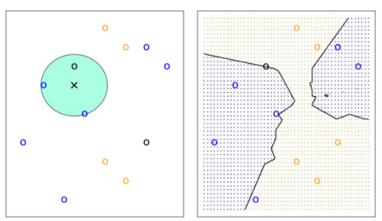
\includegraphics{cap10.png}

}

\caption{Figura 1. Límite de decisión de KNN, utilizando K = 10}

\end{Figura 1. Límite de decisión de KNN, utilizando K = 10}

\begin{Figura 2: Precisión del modelo}

{\centering 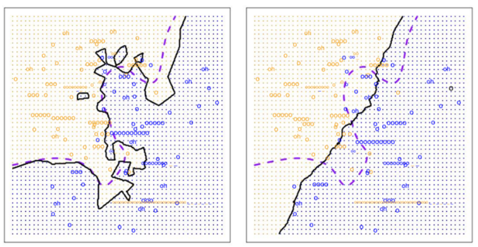
\includegraphics{cap11.png}

}

\caption{Figura 2: Precisión del modelo}

\end{Figura 2: Precisión del modelo}

Al igual que en el escenario de regresión, no existe una fuerte relación
entre la tasa de error de entrenamiento y la tasa de error de prueba.
Con K = 1, la tasa de error de entrenamiento de KNN es 0, pero la tasa
de error de prueba puede ser bastante alta. En general, a medida que
usamos métodos de clasificación más flexibles, la tasa de error de
entrenamiento disminuirá, pero es posible que no la tasa de error de
prueba. Hemos trazado la prueba KNN y los errores de entrenamiento como
una función de 1/ K. A medida que aumenta 1/K, el método se vuelve más
flexible.

Tanto en la configuración de regresión como de clasificación, elegir el
nivel correcto de flexibilidad es fundamental para el éxito de cualquier
método de aprendizaje estadístico.

\hypertarget{regresiuxf3n-lineal}{%
\subsection{\texorpdfstring{\textbf{Regresión
lineal}}{Regresión lineal}}\label{regresiuxf3n-lineal}}

la regresión lineal es una herramienta útil para predecir una respuesta
cuantitativa. Existe desde hace mucho tiempo y es el tema de
innumerables libros de texto. Además, sirve como un buen punto de
partida para nuevos enfoques: enfoques de aprendizaje, como
generalizaciones o extensiones de la regresión lineal.

\hypertarget{regresiuxf3n-lineal-simple}{%
\subsubsection{\texorpdfstring{\textbf{Regresión lineal
simple}}{Regresión lineal simple}}\label{regresiuxf3n-lineal-simple}}

Es un método directo enfocado para predecir una respuesta cuantitativa Y
sobre la base de una única variable predictora X. Supone que existe una
relación aproximadamente lineal entre X e Y. Matemáticamente, podemos
escribir esta relación lineal como:

Y = ß0 + ß1 X

Algunas veces describiremos diciendo que estamos retrocediendo Y sobre X
(o Y sobre X). ß0 y ß1 son dos constantes desconocidas que representan
los términos de intersección y pendiente en el modelo lineal. Juntos, ß0
y ß1 se conocen como los coeficientes o parámetros del modelo. Una vez
que hayamos utilizado nuestros datos de entrenamiento para producir
estimaciones podemos predecir las ventas futuras sobre la base de un
valor particular calculando.

yˆ = ߈0 + ߈1x

donde ˆy indica una predicción de Y sobre la base de X = x.

\hypertarget{estimaciuxf3n-de-los-coeficientes}{%
\subsubsection{\texorpdfstring{\textbf{Estimación de los
coeficientes}}{Estimación de los coeficientes}}\label{estimaciuxf3n-de-los-coeficientes}}

En la práctica, ß0 y ß1 son desconocidos. Por lo que, antes de que
podamos usar predicciones, debemos usar datos para estimar los
coeficientes dejar

~(x1,y1),(x2,y2),\ldots,(xn,yn),

representan n pares de observación, cada uno de los cuales consta de una
medida de X y una medida de Y. En el ejemplo de publicidad, el conjunto
de datos tiene el presupuesto de publicidad televisiva y las ventas de
productos en n = 200 mercados diferentes, lo que queremos es obtener
estimaciones de los coeficientes ߈0 y ߈1 de modo que el modelo linea
se ajuste bien a los datos disponibles.

~El i-th valor de respuesta observado y el i-th valor de respuesta que
predice nuestro modelo lineal. Definimos la suma residual de cuadrados
(RSS) como:

RSS = (y1−߈0−߈1x1) 2+(y2−߈0−߈1x2)2+···+ (yn−߈0−߈1xn) 2

~La siguiente figura se muestra el ajuste de regresión lineal simple a
los datos de publicidad, donde ߈0 = 7.03 y ߈1 = 0.0475. En otras
palabras, de acuerdo con esta aproximación, \$1,000 adicionales gastados
en publicidad televisiva están asociados con la venta de aproximadamente
47.5 unidades adicionales del producto.

En cada gráfico, el punto rojo representa el par de estimaciones de
mínimos cuadrados

\begin{Figura 3. Regresión Lineal}

{\centering 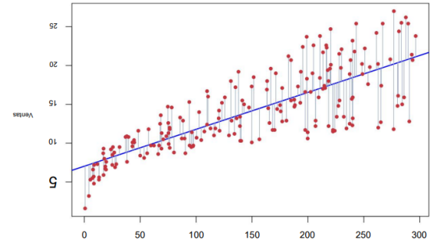
\includegraphics{cap12.png}

}

\caption{Figura 3. Regresión Lineal}

\end{Figura 3. Regresión Lineal}

\begin{Figura 4: Gráficos de contorno y tridimensionales del RSS}

{\centering 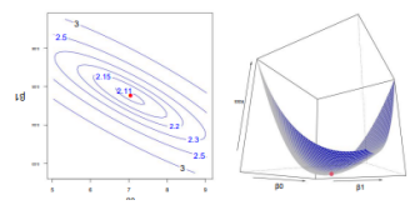
\includegraphics{cap13.png}

}

\caption{Figura 4: Gráficos de contorno y tridimensionales del RSS}

\end{Figura 4: Gráficos de contorno y tridimensionales del RSS}

\hypertarget{evaluaciuxf3n-de-la-precisiuxf3n-de-las-estimaciones-del-coeficiente}{%
\subsubsection{\texorpdfstring{\textbf{Evaluación de la precisión de las
estimaciones del
coeficiente}}{Evaluación de la precisión de las estimaciones del coeficiente}}\label{evaluaciuxf3n-de-la-precisiuxf3n-de-las-estimaciones-del-coeficiente}}

Si f se va a aproximar mediante una función lineal, entonces podemos
escribir esta relación como: Y = ß0 + ß1X + E

Aquí ß0 es el término de intersección, el término de error es un cajón
de sastre para lo que echamos de menos con este modelo simple. la
siguiente figura muestra la línea de mínimos cuadrados:

\begin{Figura 5. Línea de mínimos cuadrados}

{\centering 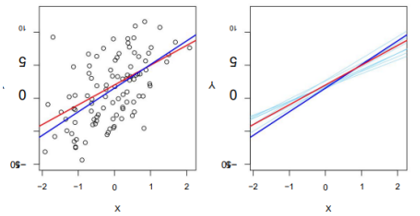
\includegraphics{cap14.png}

}

\caption{Figura 5. Línea de mínimos cuadrados}

\end{Figura 5. Línea de mínimos cuadrados}

Un conjunto de datos simulado. Izquierda: La línea roja representa la
verdadera relación, se conoce como la línea de regresión de población.
La línea azul es la línea de mínimos cuadrados; es la estimación de
mínimos cuadrados para f(X). Derecha: La línea de regresión de la
población se muestra en rojo, la línea de mínimos cuadrados en azul
oscuro y en azul claro, se muestran diez líneas de mínimos cuadrados.

\hypertarget{evaluaciuxf3n-de-la-precisiuxf3n-del-modelo-2}{%
\subsubsection{\texorpdfstring{\textbf{Evaluación de la precisión del
modelo}}{Evaluación de la precisión del modelo}}\label{evaluaciuxf3n-de-la-precisiuxf3n-del-modelo-2}}

~La calidad de un ajuste de regresión lineal generalmente se evalúa
utilizando dos cantidades relacionadas: el error estándar residual y
estadístico.

\hypertarget{error-estuxe1ndar-residual}{%
\subsubsection{\texorpdfstring{\textbf{Error estándar
residual}}{Error estándar residual}}\label{error-estuxe1ndar-residual}}

~Debido a la presencia de términos de error, incluso si conociéramos la
verdadera línea de regresión no seriamos capases de predecir
perfectamente Y a partir de X. El RSE es una estimación de la desviación
estándar de E, en generales es la cantidad promedio que la respuesta se
desviará de la verdadera línea de regresión. Se calcula usando la
fórmula.

\begin{Fórmula del error estándar residual}

{\centering 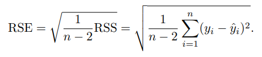
\includegraphics{f3.png}

}

\caption{Fórmula del error estándar residual}

\end{Fórmula del error estándar residual}

El RSE se considera una medida de la falta de ajuste del modelo a los
datos. Si las predicciones obtenidas con el modelo están muy cerca de
los valores reales de los resultados será pequeño y podemos concluir que
el modelo se ajusta muy bien los datos.

\hypertarget{estaduxedstica-r2}{%
\subsubsection{\texorpdfstring{\textbf{Estadística
R2}}{Estadística R2}}\label{estaduxedstica-r2}}

Proporciona una medida de ajuste alternativa. Toma la forma de una
proporción: la proporción de la varianza por lo que siempre toma un
valor entre 0 y 1, y es independiente de la escala de Y.

Se puede calcular con la siguiente fórmula:

\begin{Fórmula de estadística R2}

{\centering 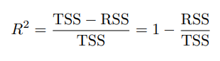
\includegraphics{f4.png}

}

\caption{Fórmula de estadística R2}

\end{Fórmula de estadística R2}

Donde TSS sumatoria es la suma total de cuadrados y mide la varianza
total en la respuesta Y y puede considerarse como la cantidad de
variabilidad inherente a la respuesta antes de que se realice la
regresión. Por el contrario, RSS mide la cantidad de variabilidad que
queda sin explicar después de realizar la regresión.

\hypertarget{regresiuxf3n-lineal-muxfaltiple}{%
\subsubsection{\texorpdfstring{\textbf{Regresión lineal
múltiple}}{Regresión lineal múltiple}}\label{regresiuxf3n-lineal-muxfaltiple}}

La regresión lineal simple es una forma útil de predecir la respuesta de
una sola variable predictora. Sin embargo, en la práctica a menudo
tenemos más de un predictor. un buen enfoque es extender un modelo de
regresión lineal simple para que pueda dar cuenta directamente de
múltiples predictores. Podemos hacer esto dando a cada predictor un
coeficiente de pendiente separado en un modelo.

\hypertarget{estimaciuxf3n-de-los-coeficientes-de-regresiuxf3n}{%
\subsubsection{\texorpdfstring{\textbf{Estimación de los coeficientes de
regresión}}{Estimación de los coeficientes de regresión}}\label{estimaciuxf3n-de-los-coeficientes-de-regresiuxf3n}}

los coeficientes de regresión ß0, ß1,\ldots, ßp suelen ser desconocidos
y deben estimarse. Dadas las estimaciones ߈0, ߈1,\ldots, ߈p, podemos
hacer predicciones usando la fórmula.

yˆ= ߈0 + ߈1x1 + ߈2x2 + ··· + ߈pxp

Los parámetros se estiman utilizando el mismo enfoque de mínimos
cuadrados.

Los valores ߈0, ߈1,\ldots, ߈p son las estimaciones del coeficiente de
regresión de mínimos cuadrados múltiples. A diferencia de las
estimaciones de regresión lineal simple dadas, las estimaciones de
coeficientes de regresión múltiple tienen formas algo complicadas que se
representan más fácilmente usando álgebra matricial.

La figura 5 muestra una tabla que muestra las estimaciones del
coeficiente de regresión múltiple cuando se utilizan los presupuestos de
publicidad en televisión, radio y periódicos para predecir.

\begin{Figura 6. Plano}

{\centering 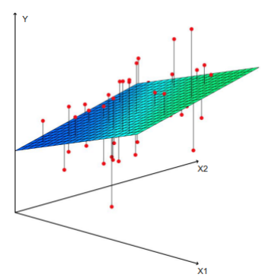
\includegraphics{cap15.png}

}

\caption{Figura 6. Plano}

\end{Figura 6. Plano}

Interpretamos estos resultados de la siguiente manera: para una cantidad
dada de publicidad en televisión y periódicos, gastar \$1,000
adicionales en publicidad por radio está asociado con aproximadamente
189 unidades de ventas adicionales.

\begin{Figura 7. Estimaciones del coeficiente de regresión múltiple}

{\centering 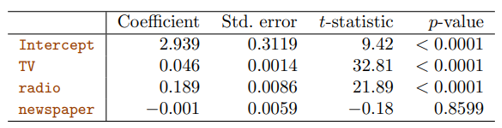
\includegraphics{cap16.png}

}

\caption{Figura 7. Estimaciones del coeficiente de regresión múltiple}

\end{Figura 7. Estimaciones del coeficiente de regresión múltiple}

\hypertarget{algunas-preguntas-importantes}{%
\subsubsection{\texorpdfstring{\textbf{Algunas preguntas
importantes}}{Algunas preguntas importantes}}\label{algunas-preguntas-importantes}}

Cuando realizamos una regresión lineal múltiple, generalmente nos
interesa responder algunas preguntas importantes.

1. ¿Es útil al menos uno de los predictores X1, X2,\ldots,Xp para
predecir la respuesta?

2. ¿Todos los predictores ayudan a explicar la utilidad de los
predictores Y?

3. ¿Qué tan bien se ajusta el modelo a los datos?

~4. Dado un conjunto de valores predictores, ¿qué valor de respuesta
deberíamos predecir? y ¿qué tan precisa es nuestra predicción?

\hypertarget{existe-una-relaciuxf3n-entre-la-respuesta-y-los-predictores}{%
\subsubsection{\texorpdfstring{\textbf{¿Existe una relación entre la
respuesta y los
predictores?}}{¿Existe una relación entre la respuesta y los predictores?}}\label{existe-una-relaciuxf3n-entre-la-respuesta-y-los-predictores}}

En la configuración de regresión lineal simple, para determinar si
existe una relación entre la respuesta y el predictor, simplemente
podemos verificar si ß1 = 0. En la configuración de regresión múltiple
con p predictores, debemos preguntarnos si todos los coeficientes de
regresión son cero.

\hypertarget{decidir-sobre-variables-importantes}{%
\subsubsection{\texorpdfstring{\textbf{Decidir sobre variables
importantes}}{Decidir sobre variables importantes}}\label{decidir-sobre-variables-importantes}}

En un análisis de regresión múltiple es calcular el estadístico F y
examinar el valor p asociado. Si concluimos sobre la base de ese valor p
que al menos uno de los predictores está relacionado con la respuesta,
entonces es natural preguntarse cuáles son los culpables. para
encontrarlos probar todos los subconjuntos posibles de los predictores
es inviable. Por lo que se necesita un modelo automatizado y un enfoque
eficiente para elegir un conjunto más pequeño de modelos a considerar.
Hay tres enfoques clásicos para esta tarea:

Selección de reenvío. Comenzamos con el modelo nulo, un modelo que
contiene un intercepto, pero no predictores. Luego ajustamos p
regresiones lineales simples y agregamos al modelo nulo la variable que
resulta en el RSS más bajo. Luego agregamos a ese modelo la variable que
resulta en el RSS más bajo para el nuevo modelo de dos variables. Este
enfoque continúa hasta que se cumple alguna regla de parada.

Selección hacia atrás. Comenzamos con todas las variables del modelo y
eliminamos la variable con el valor p más grande, es decir, la variable
que es estadísticamente menos significativa. Se ajusta el nuevo modelo
de variable (p − 1) y se elimina la variable con el valor p más grande.
Este procedimiento continúa hasta que se alcanza una regla de parada.

Selección mixta. Esta es una combinación de selección hacia adelante y
hacia atrás. Comenzamos sin variables en el modelo y, al igual que con
la selección directa, agregamos la variable que proporciona el mejor
ajuste. Continuamos agregando variables una por una, si en algún punto
el valor p de una de las variables del modelo supera cierto umbral,
eliminamos esa variable del modelo. Continuamos realizando estos pasos
hacia adelante y hacia atrás hasta que todas las variables en el modelo
tengan un valor p suficientemente bajo, y todas las variables fuera del
modelo tendrían un valor p grande si se agregaran al modelo.

\hypertarget{ajuste-del-modelo}{%
\subsubsection{\texorpdfstring{\textbf{Ajuste del
modelo}}{Ajuste del modelo}}\label{ajuste-del-modelo}}

Dos de las medidas numéricas más comunes del ajuste del modelo son RSE y
R2, la fracción de varianza explicada. Estas cantidades se calculan e
interpretan de la misma manera que para la regresión lineal simple.

Recuerde que, en la regresión simple, R2 es el cuadrado de la
correlación de la respuesta y la variable. En la regresión lineal
múltiple resulta que es igual a Cor (Y, Yˆ) ˆ2, el cuadrado de la
correlación entre la respuesta y el modelo lineal ajustado; de hecho,
una propiedad del modelo lineal ajustado es que maximiza esta
correlación entre todos los modelos lineales posibles

\hypertarget{predicciones}{%
\subsubsection{\texorpdfstring{\textbf{Predicciones}}{Predicciones}}\label{predicciones}}

Existen tres tipos de incertidumbre asociados a las predicciones.

\begin{enumerate}
\def\labelenumi{\arabic{enumi}.}
\tightlist
\item
  Las estimaciones del coeficiente ߈0, ߈1, \ldots, ߈p son
  estimaciones para ß0, ß1, \ldots, ßp. La imprecisión en las
  estimaciones de los coeficientes está relacionada con el error
  reducible. Podemos calcular un intervalo de confianza para determinar
  qué tan cerca estará Yˆ de f(X).
\item
  En la práctica asumir un modelo lineal para f(X) es casi siempre una
  aproximación a la realidad, por lo que existe una fuente adicional de
  error potencialmente reducible que llamamos sesgo del modelo.
  Entonces, cuando usamos un modelo lineal, estamos estimando la mejor
  aproximación lineal a la superficie real. aunque aquí se ignora esta
  discrepancia y se opera como si el modelo lineal fuera correcto.
\item
  Incluso si conociéramos f(X), es decir, incluso si conociéramos los
  valores verdaderos de ß0, ß1, \ldots, ßp, el valor de respuesta no se
  puede predecir perfectamente debido al error aleatorio.
\end{enumerate}

\hypertarget{otras-consideraciones-en-el-modelo-de-regresiuxf3n}{%
\subsubsection{\texorpdfstring{\textbf{Otras consideraciones en el
modelo de
regresión}}{Otras consideraciones en el modelo de regresión}}\label{otras-consideraciones-en-el-modelo-de-regresiuxf3n}}

\begin{itemize}
\item
  \textbf{Predictores cualitativos} En la práctica a menudo algunos
  predictores son cualitativos. Por ejemplo, un conjunto de datos de
  crédito se registran variables para varios titulares de tarjetas de
  crédito, la respuesta es saldo y hay varios predictores cuantitativos:
  edad, tarjetas, educación, ingresos, límite, calificación, etc.
\item
  \textbf{Predictores con solo dos niveles} Si un factor o variable
  cualitativa tiene solo dos niveles o valores posibles, podemos
  incluirla en el modelo como una variable dummy (toma dos valores
  numéricos). La decisión de cómo codificar los niveles del factor es
  arbitraria y no tiene efecto en el ajuste de la regresión, pero sí
  determina la interpretación de los coeficientes. El valor del
  coeficiente de correlación ßj correspondiente a un nivel de una
  variable dummy (codificado como 1) indica el promedio con el que
  influye dicho nivel sobre la variable respuesta en comparación con el
  nivel de referencia no codificado como variable dummy (ß0).
\item
  \textbf{Predictores cualitativos con más de dos niveles} En el caso de
  un predictor cualitativo con más de dos niveles, una sola variable
  dummy no puede representar todos los niveles posibles. En esta
  situación, podemos crear variables dummy adicionales. De nuevo, el
  nivel seleccionado como referencia es arbitrario.
\end{itemize}

\hypertarget{extensiones-del-modelo-lineal}{%
\subsubsection{\texorpdfstring{\textbf{Extensiones del Modelo
Lineal}}{Extensiones del Modelo Lineal}}\label{extensiones-del-modelo-lineal}}

El modelo de regresión lineal estándar proporciona resultados
interpretables y funciona bastante bien en muchos problemas del mundo
real. Sin embargo, hace varios supuestos altamente restrictivos. Dos de
los supuestos más importantes establecen que la relación entre los
predictores y la respuesta es aditiva y lineal. La suposición de
aditividad significa que la asociación entre un predictor X y la
respuesta Y no depende de los valores de los otros predictores. La
suposición de linealidad establece que el cambio en la respuesta Y
asociado con un cambio de una unidad en Xj es constante,
independientemente del valor de X.

\hypertarget{problemas-potenciales}{%
\subsubsection{\texorpdfstring{\textbf{Problemas
potenciales:}}{Problemas potenciales:}}\label{problemas-potenciales}}

Los más comunes entre estos son los siguientes:

\begin{enumerate}
\def\labelenumi{\arabic{enumi}.}
\tightlist
\item
  No linealidad de las relaciones respuesta-predictor.
\item
  Correlación de términos de error.
\item
  Varianza no constante de los términos de error.
\item
  Valores atípicos.
\item
  Puntos de alto apalancamiento.
\item
  Colinealidad.
\end{enumerate}

\hypertarget{no-linealidad-de-los-datos}{%
\subsubsection{\texorpdfstring{\textbf{No linealidad de los
datos}}{No linealidad de los datos}}\label{no-linealidad-de-los-datos}}

El modelo de regresión lineal supone que hay una relación lineal entre
los predictores y la respuesta. Si la verdadera relación está lejos de
ser lineal, entonces todas las conclusiones que sacamos del ajuste son
sospechosas. Los diagramas de residuos son una herramienta gráfica útil
para identificar la no linealidad.

Si la gráfica residual indica que hay asociaciones no lineales en los
datos, entonces un enfoque simple es usar transformaciones no lineales
de los predictores, como log X, √ X y X\^{}2, en el modelo de regresión.

\hypertarget{correlaciuxf3n-de-tuxe9rminos-de-error}{%
\subsubsection{\texorpdfstring{\textbf{Correlación de términos de
error}}{Correlación de términos de error}}\label{correlaciuxf3n-de-tuxe9rminos-de-error}}

Una suposición importante del modelo de regresión lineal es que los
términos de error no están correlacionados. Los errores estándar que se
calculan para los coeficientes de regresión estimados o los valores
ajustados se basan en la suposición de términos de error no
correlacionados. si los términos de error están correlacionados, podemos
tener una sensación de confianza injustificada en nuestro modelo. Para
determinar si este es el caso para un conjunto de datos determinado,
podemos trazar los residuos de nuestro modelo en función del tiempo. Si
los errores no están correlacionados, entonces no debería haber un
patrón perceptible. Por otro lado, si los términos de error están
positivamente correlacionados, podemos ver un seguimiento en los
residuos.

\hypertarget{variaciuxf3n-no-constante-de-los-tuxe9rminos-de-error}{%
\subsubsection{\texorpdfstring{\textbf{Variación no constante de los
términos de
error}}{Variación no constante de los términos de error}}\label{variaciuxf3n-no-constante-de-los-tuxe9rminos-de-error}}

en los términos de error tienen una varianza constante. Los errores
estándar, los intervalos de confianza y las pruebas de hipótesis
asociadas con el modelo lineal se basan en esta suposición.
Desafortunadamente, a menudo ocurre que las varianzas de los términos de
error no son constantes. Las varianzas de los términos de error pueden
aumentar con el valor de la respuesta. Se pueden identificar varianzas
no constantes en los errores, o heteroscedasticidad, en estos problemas,
una posible solución es transformar la respuesta Y utilizando una
función cóncava como log Y o √ Y. Transformación que da como resultado
una mayor cantidad de reducción de las respuestas más grandes, lo que
conduce a una reducción de la heteroscedasticidad.

\hypertarget{valores-atuxedpicos}{%
\subsubsection{\texorpdfstring{\textbf{Valores
atípicos}}{Valores atípicos}}\label{valores-atuxedpicos}}

Es un punto para el cual yi está lejos del valor predicho por el modelo.
Los valores atípicos pueden surgir por una variedad de razones, como el
registro incorrecto de una observación durante la recopilación de datos.
Los gráficos residuales se pueden utilizar para identificar valores
atípicos. Para abordar este problema, en lugar de graficar los residuos,
podemos graficar los residuos, calculados al dividir cada residuo ei por
su error estándar estimado. Las observaciones cuyos residuos son mayores
que 3 en valor absoluto son posibles valores atípicos. Si creemos que se
ha producido un valor atípico debido a un error en la recopilación o
registro de datos, entonces una solución es simplemente eliminar la
observación.

\hypertarget{altos-puntos-de-apalancamiento}{%
\subsubsection{\texorpdfstring{\textbf{Altos puntos de
apalancamiento}}{Altos puntos de apalancamiento}}\label{altos-puntos-de-apalancamiento}}

Las observaciones con alto apalancamiento tienen un valor inusual para
xi, las observaciones de alto apalancamiento tienden a tener un impacto
considerable en la línea de regresión estimada. Es motivo de
preocupación si la línea de mínimos cuadrados se ve muy afectada por
solo un par de observaciones, porque cualquier problema con estos puntos
puede invalidar todo el ajuste. Por esta razón, es importante
identificar observaciones de alto apalancamiento. En una regresión
lineal simple, las observaciones de alto apalancamiento son bastante
fáciles de identificar, ya que simplemente podemos buscar observaciones
para las cuales el valor del predictor está fuera del rango normal de
las observaciones.

\hypertarget{colinealidad}{%
\subsubsection{\texorpdfstring{\textbf{Colinealidad}}{Colinealidad}}\label{colinealidad}}

se refiere a la situación en la que dos o más variables predictoras
están estrechamente relacionadas entre sí. Identificar y abordar los
posibles problemas de colinealidad al ajustar el modelo es de suma
importancia para no tener problemas, una forma de detectar la
colinealidad es observar la matriz de correlación de los predictores. Un
elemento de esta matriz que es grande en valor absoluto indica un par de
variables altamente correlacionadas y, por lo tanto, un problema de
colinealidad en los datos. Desafortunadamente, no todos los problemas de
colinealidad pueden detectarse mediante la inspección de la matriz de
correlación: es posible que exista colinealidad entre tres o más
variables incluso si ningún par de variables tiene una correlación
particularmente alta. A esta situación la llamamos multicolinealidad.

\hypertarget{comparaciuxf3n-de-regresiuxf3n-lineal-con-k-vecinos-muxe1s-cercanos}{%
\subsubsection{\texorpdfstring{\textbf{Comparación de regresión lineal
con K-vecinos más
cercanos}}{Comparación de regresión lineal con K-vecinos más cercanos}}\label{comparaciuxf3n-de-regresiuxf3n-lineal-con-k-vecinos-muxe1s-cercanos}}

La regresión lineal es un ejemplo de un método paramétrico porque asume
una forma funcional lineal de f(X). La ventaja es que, por lo general,
son fáciles de configurar, ya que solo se necesita evaluar una pequeña
cantidad de coeficientes. En el caso de la regresión lineal, los
coeficientes son fáciles de interpretar y su significancia estadística
puede probarse fácilmente. Pero los métodos paramétricos tienen un
inconveniente: por diseño, hacen fuertes suposiciones sobre la forma de
f(X). Si la forma de la función especificada está lejos de hecho, si
nuestro objetivo es la precisión predictiva, los métodos paramétricos
funcionarán mal. Por el contrario, los métodos no paramétricos no tienen
una forma bien definida. Por lo tanto, la parametrización de f (X)
proporciona una forma alternativa y más flexible realizar la regresión.

El método de regresión KNN está estrechamente relacionado con el
clasificador KNN. Dado un valor para K y un punto de predicción x0, la
regresión KNN primero identifica las observaciones de entrenamiento K
más cercanas a x0, representadas por N0. Luego estima f(x0) usando el
promedio de todas las respuestas de entrenamiento en N0.

\begin{Fórmula de regresión KNN}

{\centering 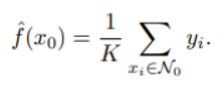
\includegraphics{f5.png}

}

\caption{Fórmula de regresión KNN}

\end{Fórmula de regresión KNN}

La figura ilustra dos ajustes KNN en un conjunto de datos con p = 2
predictores. El ajuste con K = 1 se muestra en el panel de la izquierda,
mientras que el panel de la derecha corresponde a K = 9. Vemos que
cuando K = 1, el ajuste KNN interpola perfectamente las observaciones de
entrenamiento y, en consecuencia, toma la forma de una función de paso.
Cuando K = 9, el ajuste KNN sigue siendo una función escalonada, pero el
promedio de nueve observaciones da como resultado regiones mucho más
pequeñas de constante predicción y, en consecuencia, un ajuste más
suave. El valor óptimo de K dependerá del compromiso sesgo-varianza, un
valor pequeño de K proporciona el ajuste más flexible, que tendrá un
sesgo bajo, pero una varianza alta. Esta varianza se debe al hecho de
que la predicción en una región dada depende completamente de una sola
observación. Caso contrario, los valores más grandes de K proporcionan
un ajuste más suave y menos variable; la predicción en una región es un
promedio de varios puntos, por lo que cambiar una observación tiene un
efecto menor. Sin embargo, el suavizado puede causar un sesgo al
enmascarar parte de la estructura en f(X).

\begin{Figura 8. Ajuste KNN}

{\centering 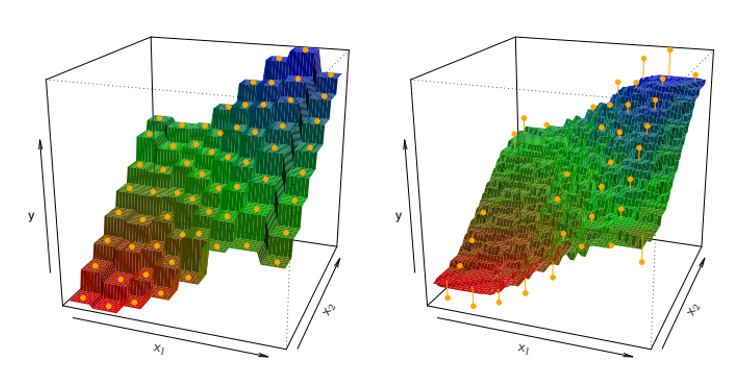
\includegraphics{cap17.png}

}

\caption{Figura 8. Ajuste KNN}

\end{Figura 8. Ajuste KNN}

En general, el valor óptimo de K dependerá del equilibrio entre sesgo y
varianza, que introdujimos en el capítulo 2. Un valor pequeño de K
proporciona el ajuste más flexible, que tendrá un sesgo bajo, pero una
varianza alta. Esta varianza se debe al hecho de que la predicción en
una región dada depende totalmente de una sola observación. La
predicción en una región es una media de varios puntos, por lo que el
cambio de una observación tiene un efecto menor.

\hypertarget{laboratorio-unidad-3}{%
\subsubsection{Laboratorio Unidad 3}\label{laboratorio-unidad-3}}

Para esta parte del ejemplo se debe instalar la librería gmodels para
los cual se puede utilizar el comando: (install.packages(``MASS''),
install.packages(``ISLR2''), install.packages(``ISLR2'')).

\begin{Shaded}
\begin{Highlighting}[]
\FunctionTok{library}\NormalTok{ (MASS)}
\FunctionTok{library}\NormalTok{ (ISLR2)}
\end{Highlighting}
\end{Shaded}

\begin{verbatim}

Attaching package: 'ISLR2'
\end{verbatim}

\begin{verbatim}
The following object is masked from 'package:MASS':

    Boston
\end{verbatim}

\begin{Shaded}
\begin{Highlighting}[]
\FunctionTok{library}\NormalTok{ (faraway)}
\end{Highlighting}
\end{Shaded}

La biblioteca ISLR2 contiene el conjunto de datos de Boston, que
registra medv (valor medio de la casa) para 506 distritos censales en
Boston. Buscaremos predecir medv usando 12 predictores como rm (número
promedio de habitaciones por casa), age (edad promedio de las casas) y
lstat (porcentaje de hogares con bajo estatus socioeconómico).

\begin{Shaded}
\begin{Highlighting}[]
\FunctionTok{head}\NormalTok{ (Boston)}
\end{Highlighting}
\end{Shaded}

\begin{verbatim}
     crim zn indus chas   nox    rm  age    dis rad tax ptratio lstat medv
1 0.00632 18  2.31    0 0.538 6.575 65.2 4.0900   1 296    15.3  4.98 24.0
2 0.02731  0  7.07    0 0.469 6.421 78.9 4.9671   2 242    17.8  9.14 21.6
3 0.02729  0  7.07    0 0.469 7.185 61.1 4.9671   2 242    17.8  4.03 34.7
4 0.03237  0  2.18    0 0.458 6.998 45.8 6.0622   3 222    18.7  2.94 33.4
5 0.06905  0  2.18    0 0.458 7.147 54.2 6.0622   3 222    18.7  5.33 36.2
6 0.02985  0  2.18    0 0.458 6.430 58.7 6.0622   3 222    18.7  5.21 28.7
\end{verbatim}

\begin{Shaded}
\begin{Highlighting}[]
\NormalTok{lm.fit }\OtherTok{\textless{}{-}} \FunctionTok{lm}\NormalTok{(medv }\SpecialCharTok{\textasciitilde{}}\NormalTok{ lstat, }\AttributeTok{data =}\NormalTok{ Boston)}
\FunctionTok{attach}\NormalTok{ (Boston)}
\NormalTok{lm.fit }\OtherTok{\textless{}{-}} \FunctionTok{lm}\NormalTok{(medv }\SpecialCharTok{\textasciitilde{}}\NormalTok{ lstat)}
\end{Highlighting}
\end{Shaded}

Se realizó el cambio de posición del código que aparese a continuación
para que este no tuviera ningún error porque el mismo no se encontraba
definido.

\begin{Shaded}
\begin{Highlighting}[]
\NormalTok{lm.fit }
\end{Highlighting}
\end{Shaded}

\begin{verbatim}

Call:
lm(formula = medv ~ lstat)

Coefficients:
(Intercept)        lstat  
      34.55        -0.95  
\end{verbatim}

\begin{Shaded}
\begin{Highlighting}[]
\FunctionTok{summary}\NormalTok{(lm.fit)}
\end{Highlighting}
\end{Shaded}

\begin{verbatim}

Call:
lm(formula = medv ~ lstat)

Residuals:
    Min      1Q  Median      3Q     Max 
-15.168  -3.990  -1.318   2.034  24.500 

Coefficients:
            Estimate Std. Error t value Pr(>|t|)    
(Intercept) 34.55384    0.56263   61.41   <2e-16 ***
lstat       -0.95005    0.03873  -24.53   <2e-16 ***
---
Signif. codes:  0 '***' 0.001 '**' 0.01 '*' 0.05 '.' 0.1 ' ' 1

Residual standard error: 6.216 on 504 degrees of freedom
Multiple R-squared:  0.5441,    Adjusted R-squared:  0.5432 
F-statistic: 601.6 on 1 and 504 DF,  p-value: < 2.2e-16
\end{verbatim}

\begin{Shaded}
\begin{Highlighting}[]
\FunctionTok{names}\NormalTok{ (lm.fit)}
\end{Highlighting}
\end{Shaded}

\begin{verbatim}
 [1] "coefficients"  "residuals"     "effects"       "rank"         
 [5] "fitted.values" "assign"        "qr"            "df.residual"  
 [9] "xlevels"       "call"          "terms"         "model"        
\end{verbatim}

\begin{Shaded}
\begin{Highlighting}[]
\FunctionTok{coef}\NormalTok{ (lm.fit)}
\end{Highlighting}
\end{Shaded}

\begin{verbatim}
(Intercept)       lstat 
 34.5538409  -0.9500494 
\end{verbatim}

\begin{Shaded}
\begin{Highlighting}[]
\FunctionTok{confint}\NormalTok{(lm.fit)}
\end{Highlighting}
\end{Shaded}

\begin{verbatim}
                2.5 %     97.5 %
(Intercept) 33.448457 35.6592247
lstat       -1.026148 -0.8739505
\end{verbatim}

\begin{Shaded}
\begin{Highlighting}[]
\FunctionTok{predict}\NormalTok{(lm.fit, }\FunctionTok{data.frame}\NormalTok{(}\AttributeTok{lstat =}\NormalTok{ (}\FunctionTok{c}\NormalTok{(}\DecValTok{5}\NormalTok{,}\DecValTok{10}\NormalTok{,}\DecValTok{15}\NormalTok{))),}
        \AttributeTok{interval =} \StringTok{"confidence"}\NormalTok{)}
\end{Highlighting}
\end{Shaded}

\begin{verbatim}
       fit      lwr      upr
1 29.80359 29.00741 30.59978
2 25.05335 24.47413 25.63256
3 20.30310 19.73159 20.87461
\end{verbatim}

\begin{Shaded}
\begin{Highlighting}[]
\FunctionTok{predict}\NormalTok{(lm.fit, }\FunctionTok{data.frame}\NormalTok{(}\AttributeTok{lstat =}\NormalTok{ (}\FunctionTok{c}\NormalTok{(}\DecValTok{5}\NormalTok{,}\DecValTok{10}\NormalTok{,}\DecValTok{15}\NormalTok{))),}
        \AttributeTok{interval =} \StringTok{"prediction"}\NormalTok{)}
\end{Highlighting}
\end{Shaded}

\begin{verbatim}
       fit       lwr      upr
1 29.80359 17.565675 42.04151
2 25.05335 12.827626 37.27907
3 20.30310  8.077742 32.52846
\end{verbatim}

\begin{Shaded}
\begin{Highlighting}[]
\FunctionTok{plot}\NormalTok{ (lstat , medv)}
\FunctionTok{abline}\NormalTok{ (lm.fit)}
\end{Highlighting}
\end{Shaded}

\begin{figure}[H]

{\centering 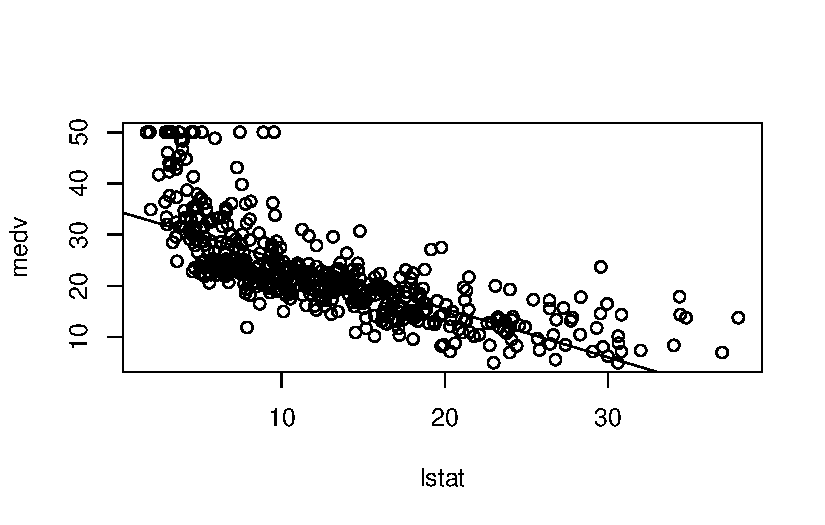
\includegraphics{Regresion-lineal-simple-y-multiple_files/figure-pdf/unnamed-chunk-11-1.pdf}

}

\end{figure}

\begin{Shaded}
\begin{Highlighting}[]
\FunctionTok{plot}\NormalTok{(lstat, medv)}
\FunctionTok{abline}\NormalTok{ (lm.fit , }\AttributeTok{lwd =} \DecValTok{3}\NormalTok{)}
\FunctionTok{abline}\NormalTok{ (lm.fit , }\AttributeTok{lwd =} \DecValTok{3}\NormalTok{, }\AttributeTok{col =} \StringTok{" red "}\NormalTok{)}
\end{Highlighting}
\end{Shaded}

\begin{figure}[H]

{\centering 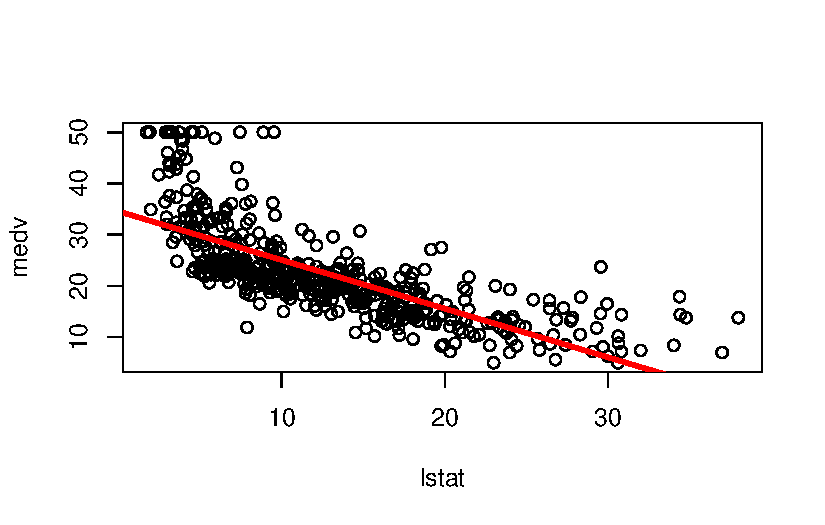
\includegraphics{Regresion-lineal-simple-y-multiple_files/figure-pdf/unnamed-chunk-12-1.pdf}

}

\end{figure}

\begin{Shaded}
\begin{Highlighting}[]
\FunctionTok{plot}\NormalTok{ (lstat , medv , }\AttributeTok{col =} \StringTok{" red "}\NormalTok{)}
\end{Highlighting}
\end{Shaded}

\begin{figure}[H]

{\centering 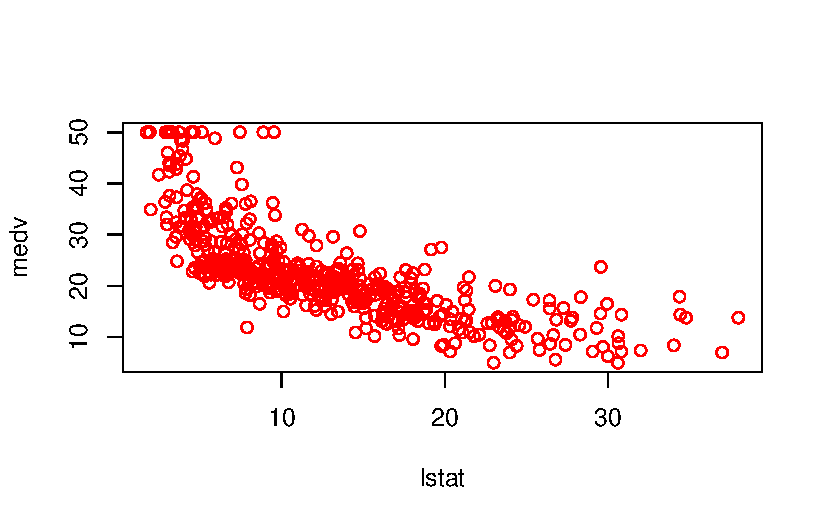
\includegraphics{Regresion-lineal-simple-y-multiple_files/figure-pdf/unnamed-chunk-12-2.pdf}

}

\end{figure}

\begin{Shaded}
\begin{Highlighting}[]
\FunctionTok{plot}\NormalTok{ (lstat , medv , }\AttributeTok{pch =} \DecValTok{20}\NormalTok{)}
\end{Highlighting}
\end{Shaded}

\begin{figure}[H]

{\centering 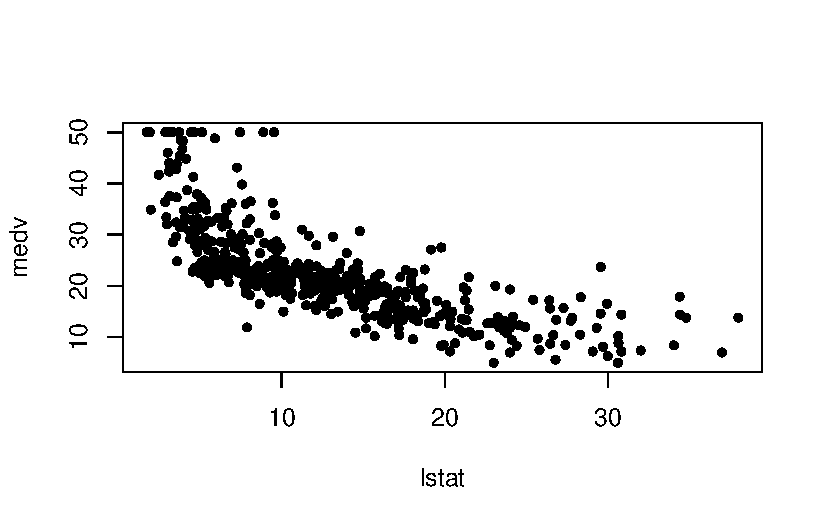
\includegraphics{Regresion-lineal-simple-y-multiple_files/figure-pdf/unnamed-chunk-12-3.pdf}

}

\end{figure}

\begin{Shaded}
\begin{Highlighting}[]
\FunctionTok{plot}\NormalTok{ (lstat , medv , }\AttributeTok{pch =} \StringTok{"+"}\NormalTok{)}
\end{Highlighting}
\end{Shaded}

\begin{figure}[H]

{\centering 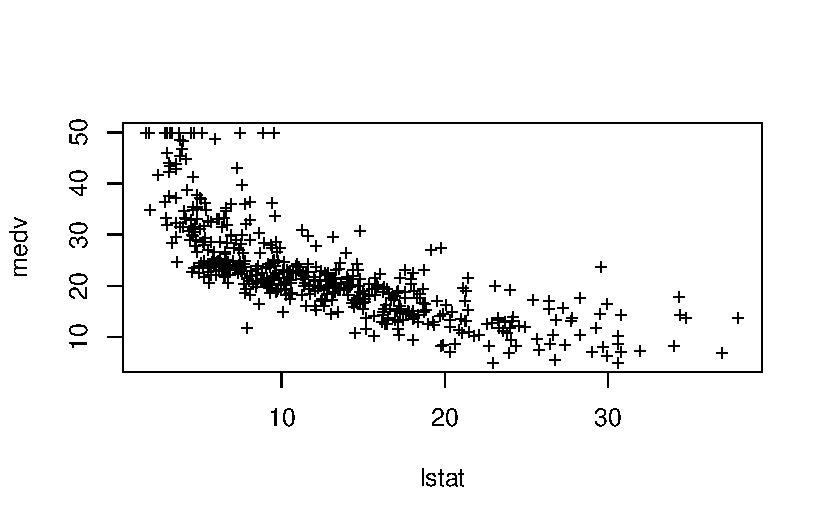
\includegraphics{Regresion-lineal-simple-y-multiple_files/figure-pdf/unnamed-chunk-12-4.pdf}

}

\end{figure}

\begin{Shaded}
\begin{Highlighting}[]
\FunctionTok{plot}\NormalTok{ (}\DecValTok{1}\SpecialCharTok{:}\DecValTok{20}\NormalTok{, }\DecValTok{1}\SpecialCharTok{:}\DecValTok{20}\NormalTok{, }\AttributeTok{pch =} \DecValTok{1}\SpecialCharTok{:}\DecValTok{20}\NormalTok{)}
\end{Highlighting}
\end{Shaded}

\begin{figure}[H]

{\centering 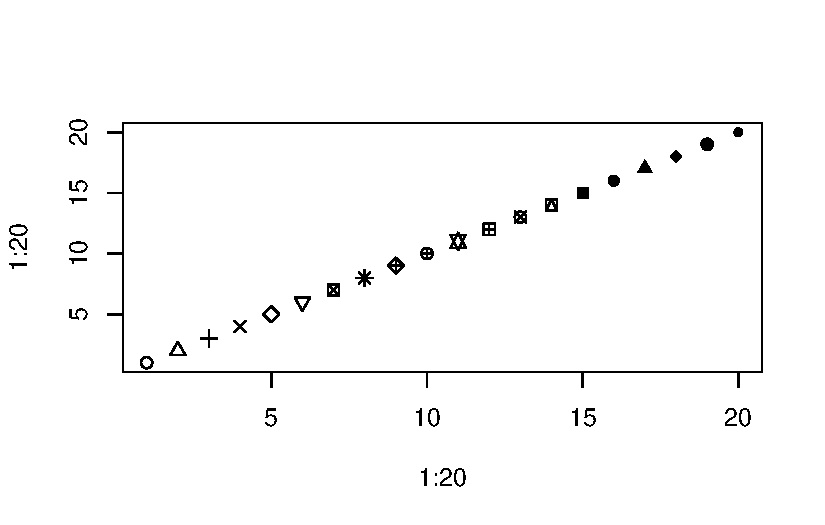
\includegraphics{Regresion-lineal-simple-y-multiple_files/figure-pdf/unnamed-chunk-12-5.pdf}

}

\end{figure}

\begin{Shaded}
\begin{Highlighting}[]
\FunctionTok{par}\NormalTok{ (}\AttributeTok{mfrow =} \FunctionTok{c}\NormalTok{(}\DecValTok{2}\NormalTok{, }\DecValTok{2}\NormalTok{))}
\FunctionTok{plot}\NormalTok{ (lm.fit)}
\end{Highlighting}
\end{Shaded}

\begin{figure}[H]

{\centering 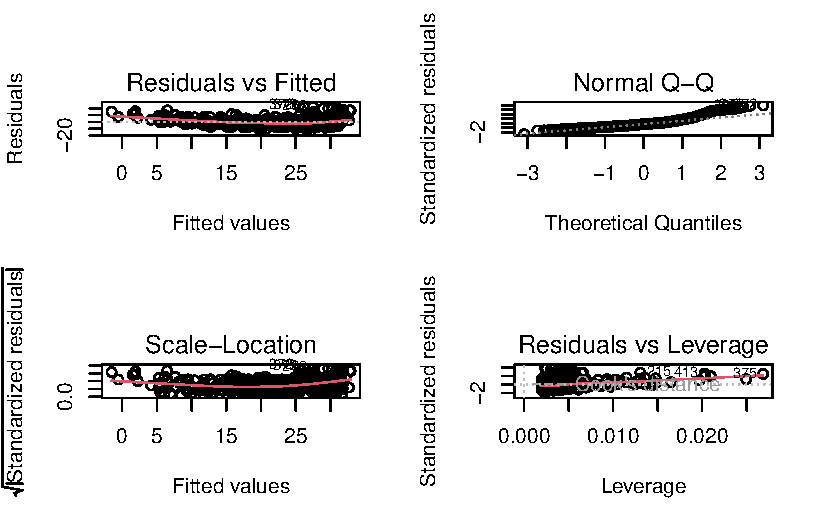
\includegraphics{Regresion-lineal-simple-y-multiple_files/figure-pdf/unnamed-chunk-13-1.pdf}

}

\end{figure}

\begin{Shaded}
\begin{Highlighting}[]
\FunctionTok{plot}\NormalTok{ ( }\FunctionTok{predict}\NormalTok{ (lm.fit), }\FunctionTok{residuals}\NormalTok{ (lm.fit))}
\end{Highlighting}
\end{Shaded}

\begin{figure}[H]

{\centering 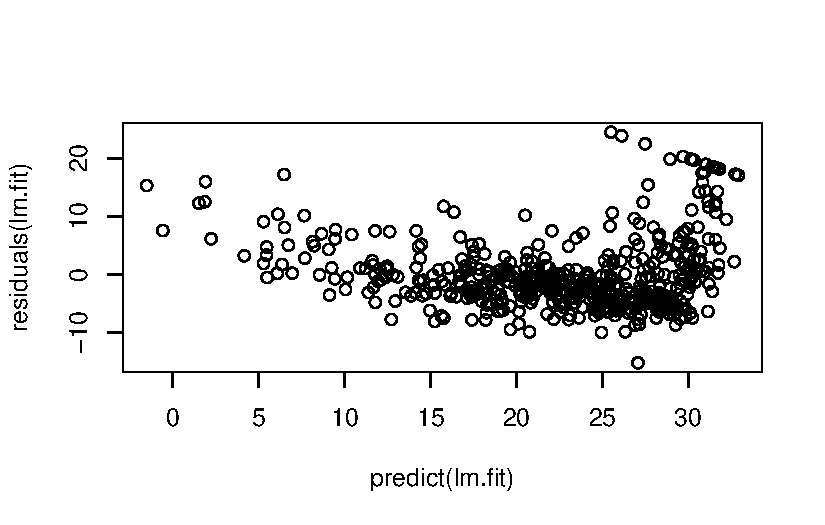
\includegraphics{Regresion-lineal-simple-y-multiple_files/figure-pdf/unnamed-chunk-14-1.pdf}

}

\end{figure}

\begin{Shaded}
\begin{Highlighting}[]
\FunctionTok{plot}\NormalTok{ ( }\FunctionTok{predict}\NormalTok{ (lm.fit), }\FunctionTok{rstudent}\NormalTok{ (lm.fit))}
\end{Highlighting}
\end{Shaded}

\begin{figure}[H]

{\centering 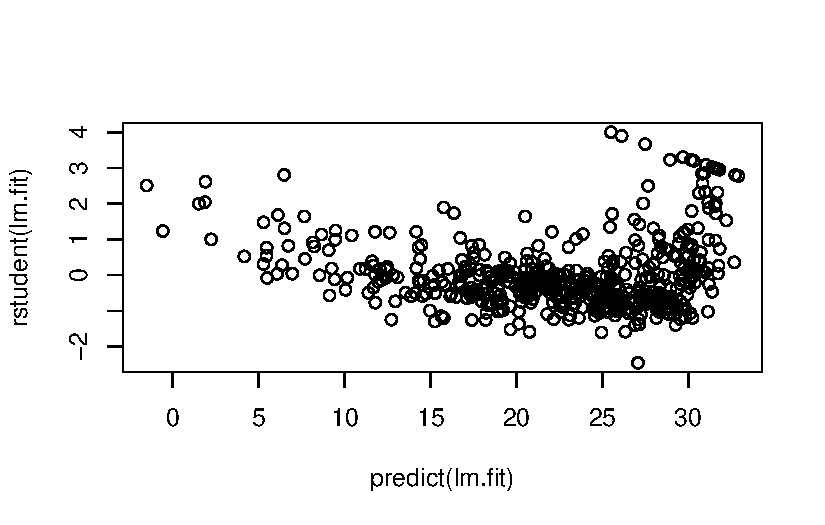
\includegraphics{Regresion-lineal-simple-y-multiple_files/figure-pdf/unnamed-chunk-14-2.pdf}

}

\end{figure}

\begin{Shaded}
\begin{Highlighting}[]
\FunctionTok{plot}\NormalTok{ ( }\FunctionTok{hatvalues}\NormalTok{ (lm.fit))}
\end{Highlighting}
\end{Shaded}

\begin{figure}[H]

{\centering 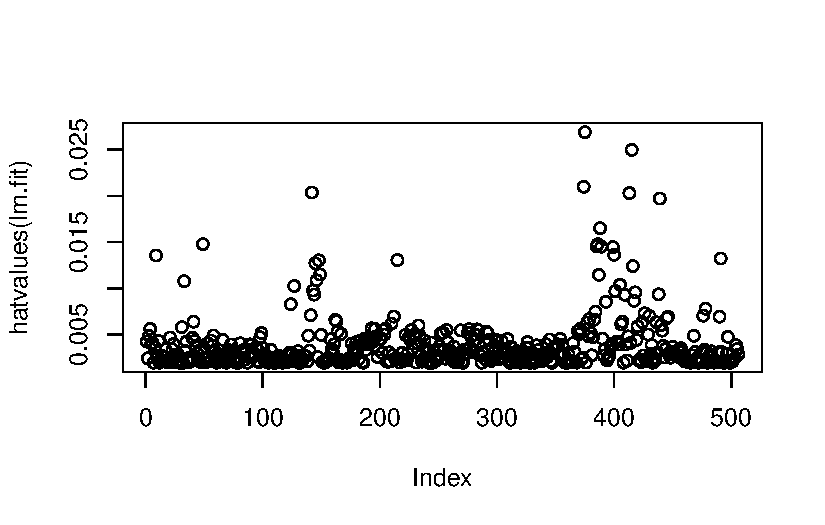
\includegraphics{Regresion-lineal-simple-y-multiple_files/figure-pdf/unnamed-chunk-15-1.pdf}

}

\end{figure}

\begin{Shaded}
\begin{Highlighting}[]
\FunctionTok{which.max}\NormalTok{ ( }\FunctionTok{hatvalues}\NormalTok{ (lm.fit))}
\end{Highlighting}
\end{Shaded}

\begin{verbatim}
375 
375 
\end{verbatim}

\textbf{Regresión Lineal Múltiple}

\begin{Shaded}
\begin{Highlighting}[]
\NormalTok{lm.fit }\OtherTok{\textless{}{-}} \FunctionTok{lm}\NormalTok{(medv }\SpecialCharTok{\textasciitilde{}}\NormalTok{ lstat }\SpecialCharTok{+}\NormalTok{ age , }\AttributeTok{data =}\NormalTok{ Boston)}
\FunctionTok{summary}\NormalTok{ (lm.fit)}
\end{Highlighting}
\end{Shaded}

\begin{verbatim}

Call:
lm(formula = medv ~ lstat + age, data = Boston)

Residuals:
    Min      1Q  Median      3Q     Max 
-15.981  -3.978  -1.283   1.968  23.158 

Coefficients:
            Estimate Std. Error t value Pr(>|t|)    
(Intercept) 33.22276    0.73085  45.458  < 2e-16 ***
lstat       -1.03207    0.04819 -21.416  < 2e-16 ***
age          0.03454    0.01223   2.826  0.00491 ** 
---
Signif. codes:  0 '***' 0.001 '**' 0.01 '*' 0.05 '.' 0.1 ' ' 1

Residual standard error: 6.173 on 503 degrees of freedom
Multiple R-squared:  0.5513,    Adjusted R-squared:  0.5495 
F-statistic:   309 on 2 and 503 DF,  p-value: < 2.2e-16
\end{verbatim}

\begin{Shaded}
\begin{Highlighting}[]
\NormalTok{lm.fit }\OtherTok{\textless{}{-}} \FunctionTok{lm}\NormalTok{(medv }\SpecialCharTok{\textasciitilde{}}\NormalTok{ ., }\AttributeTok{data =}\NormalTok{ Boston)}
\FunctionTok{summary}\NormalTok{ (lm.fit)}
\end{Highlighting}
\end{Shaded}

\begin{verbatim}

Call:
lm(formula = medv ~ ., data = Boston)

Residuals:
     Min       1Q   Median       3Q      Max 
-15.1304  -2.7673  -0.5814   1.9414  26.2526 

Coefficients:
              Estimate Std. Error t value Pr(>|t|)    
(Intercept)  41.617270   4.936039   8.431 3.79e-16 ***
crim         -0.121389   0.033000  -3.678 0.000261 ***
zn            0.046963   0.013879   3.384 0.000772 ***
indus         0.013468   0.062145   0.217 0.828520    
chas          2.839993   0.870007   3.264 0.001173 ** 
nox         -18.758022   3.851355  -4.870 1.50e-06 ***
rm            3.658119   0.420246   8.705  < 2e-16 ***
age           0.003611   0.013329   0.271 0.786595    
dis          -1.490754   0.201623  -7.394 6.17e-13 ***
rad           0.289405   0.066908   4.325 1.84e-05 ***
tax          -0.012682   0.003801  -3.337 0.000912 ***
ptratio      -0.937533   0.132206  -7.091 4.63e-12 ***
lstat        -0.552019   0.050659 -10.897  < 2e-16 ***
---
Signif. codes:  0 '***' 0.001 '**' 0.01 '*' 0.05 '.' 0.1 ' ' 1

Residual standard error: 4.798 on 493 degrees of freedom
Multiple R-squared:  0.7343,    Adjusted R-squared:  0.7278 
F-statistic: 113.5 on 12 and 493 DF,  p-value: < 2.2e-16
\end{verbatim}

\begin{Shaded}
\begin{Highlighting}[]
\FunctionTok{library}\NormalTok{ (car)}
\end{Highlighting}
\end{Shaded}

\begin{verbatim}
Loading required package: carData
\end{verbatim}

\begin{verbatim}

Attaching package: 'car'
\end{verbatim}

\begin{verbatim}
The following objects are masked from 'package:faraway':

    logit, vif
\end{verbatim}

\begin{Shaded}
\begin{Highlighting}[]
\FunctionTok{vif}\NormalTok{ (lm.fit)}
\end{Highlighting}
\end{Shaded}

\begin{verbatim}
    crim       zn    indus     chas      nox       rm      age      dis 
1.767486 2.298459 3.987181 1.071168 4.369093 1.912532 3.088232 3.954037 
     rad      tax  ptratio    lstat 
7.445301 9.002158 1.797060 2.870777 
\end{verbatim}

\begin{Shaded}
\begin{Highlighting}[]
\NormalTok{lm.fit1 }\OtherTok{\textless{}{-}} \FunctionTok{lm}\NormalTok{(medv }\SpecialCharTok{\textasciitilde{}}\NormalTok{ . }\SpecialCharTok{{-}}\NormalTok{ age , }\AttributeTok{data =}\NormalTok{ Boston)}
\FunctionTok{summary}\NormalTok{ (lm.fit1)}
\end{Highlighting}
\end{Shaded}

\begin{verbatim}

Call:
lm(formula = medv ~ . - age, data = Boston)

Residuals:
     Min       1Q   Median       3Q      Max 
-15.1851  -2.7330  -0.6116   1.8555  26.3838 

Coefficients:
              Estimate Std. Error t value Pr(>|t|)    
(Intercept)  41.525128   4.919684   8.441 3.52e-16 ***
crim         -0.121426   0.032969  -3.683 0.000256 ***
zn            0.046512   0.013766   3.379 0.000785 ***
indus         0.013451   0.062086   0.217 0.828577    
chas          2.852773   0.867912   3.287 0.001085 ** 
nox         -18.485070   3.713714  -4.978 8.91e-07 ***
rm            3.681070   0.411230   8.951  < 2e-16 ***
dis          -1.506777   0.192570  -7.825 3.12e-14 ***
rad           0.287940   0.066627   4.322 1.87e-05 ***
tax          -0.012653   0.003796  -3.333 0.000923 ***
ptratio      -0.934649   0.131653  -7.099 4.39e-12 ***
lstat        -0.547409   0.047669 -11.483  < 2e-16 ***
---
Signif. codes:  0 '***' 0.001 '**' 0.01 '*' 0.05 '.' 0.1 ' ' 1

Residual standard error: 4.794 on 494 degrees of freedom
Multiple R-squared:  0.7343,    Adjusted R-squared:  0.7284 
F-statistic: 124.1 on 11 and 494 DF,  p-value: < 2.2e-16
\end{verbatim}

\begin{Shaded}
\begin{Highlighting}[]
\NormalTok{ lm.fit1 }\OtherTok{\textless{}{-}} \FunctionTok{update}\NormalTok{ (lm.fit , }\SpecialCharTok{\textasciitilde{}}\NormalTok{ . }\SpecialCharTok{{-}}\NormalTok{ age)}
\end{Highlighting}
\end{Shaded}

\begin{Shaded}
\begin{Highlighting}[]
\FunctionTok{summary}\NormalTok{ (}\FunctionTok{lm}\NormalTok{(medv }\SpecialCharTok{\textasciitilde{}}\NormalTok{ lstat }\SpecialCharTok{*}\NormalTok{ age , }\AttributeTok{data =}\NormalTok{ Boston))}
\end{Highlighting}
\end{Shaded}

\begin{verbatim}

Call:
lm(formula = medv ~ lstat * age, data = Boston)

Residuals:
    Min      1Q  Median      3Q     Max 
-15.806  -4.045  -1.333   2.085  27.552 

Coefficients:
              Estimate Std. Error t value Pr(>|t|)    
(Intercept) 36.0885359  1.4698355  24.553  < 2e-16 ***
lstat       -1.3921168  0.1674555  -8.313 8.78e-16 ***
age         -0.0007209  0.0198792  -0.036   0.9711    
lstat:age    0.0041560  0.0018518   2.244   0.0252 *  
---
Signif. codes:  0 '***' 0.001 '**' 0.01 '*' 0.05 '.' 0.1 ' ' 1

Residual standard error: 6.149 on 502 degrees of freedom
Multiple R-squared:  0.5557,    Adjusted R-squared:  0.5531 
F-statistic: 209.3 on 3 and 502 DF,  p-value: < 2.2e-16
\end{verbatim}

\begin{Shaded}
\begin{Highlighting}[]
\NormalTok{lm.fit2 }\OtherTok{\textless{}{-}} \FunctionTok{lm}\NormalTok{(medv }\SpecialCharTok{\textasciitilde{}}\NormalTok{ lstat }\SpecialCharTok{+} \FunctionTok{I}\NormalTok{(lstat}\SpecialCharTok{\^{}}\DecValTok{2}\NormalTok{))}
\FunctionTok{summary}\NormalTok{ (lm.fit2)}
\end{Highlighting}
\end{Shaded}

\begin{verbatim}

Call:
lm(formula = medv ~ lstat + I(lstat^2))

Residuals:
     Min       1Q   Median       3Q      Max 
-15.2834  -3.8313  -0.5295   2.3095  25.4148 

Coefficients:
             Estimate Std. Error t value Pr(>|t|)    
(Intercept) 42.862007   0.872084   49.15   <2e-16 ***
lstat       -2.332821   0.123803  -18.84   <2e-16 ***
I(lstat^2)   0.043547   0.003745   11.63   <2e-16 ***
---
Signif. codes:  0 '***' 0.001 '**' 0.01 '*' 0.05 '.' 0.1 ' ' 1

Residual standard error: 5.524 on 503 degrees of freedom
Multiple R-squared:  0.6407,    Adjusted R-squared:  0.6393 
F-statistic: 448.5 on 2 and 503 DF,  p-value: < 2.2e-16
\end{verbatim}

\begin{Shaded}
\begin{Highlighting}[]
\NormalTok{lm.fit }\OtherTok{\textless{}{-}} \FunctionTok{lm}\NormalTok{(medv }\SpecialCharTok{\textasciitilde{}}\NormalTok{ lstat)}
\FunctionTok{anova}\NormalTok{ (lm.fit , lm.fit2)}
\end{Highlighting}
\end{Shaded}

\begin{verbatim}
Analysis of Variance Table

Model 1: medv ~ lstat
Model 2: medv ~ lstat + I(lstat^2)
  Res.Df   RSS Df Sum of Sq     F    Pr(>F)    
1    504 19472                                 
2    503 15347  1    4125.1 135.2 < 2.2e-16 ***
---
Signif. codes:  0 '***' 0.001 '**' 0.01 '*' 0.05 '.' 0.1 ' ' 1
\end{verbatim}

\begin{Shaded}
\begin{Highlighting}[]
\FunctionTok{par}\NormalTok{ (}\AttributeTok{mfrow =} \FunctionTok{c}\NormalTok{(}\DecValTok{2}\NormalTok{, }\DecValTok{2}\NormalTok{))}
\FunctionTok{plot}\NormalTok{ (lm.fit2)}
\end{Highlighting}
\end{Shaded}

\begin{figure}[H]

{\centering 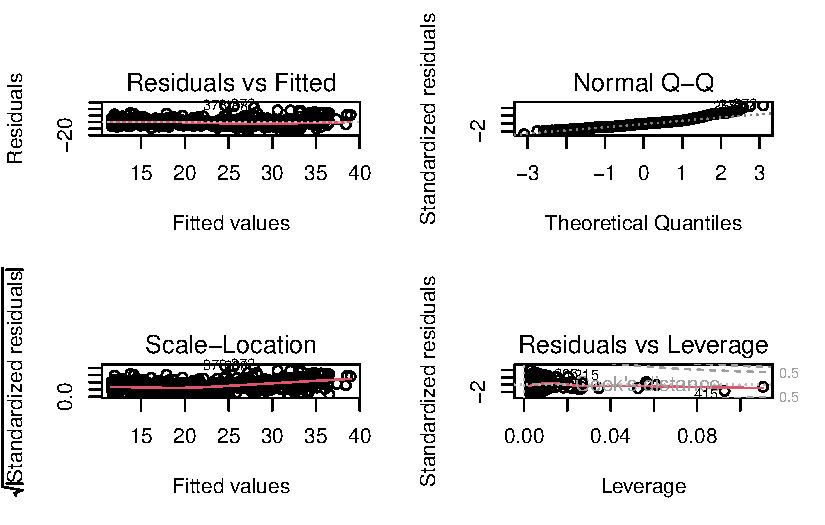
\includegraphics{Regresion-lineal-simple-y-multiple_files/figure-pdf/unnamed-chunk-24-1.pdf}

}

\end{figure}

\begin{Shaded}
\begin{Highlighting}[]
\NormalTok{lm.fit5 }\OtherTok{\textless{}{-}} \FunctionTok{lm}\NormalTok{(medv }\SpecialCharTok{\textasciitilde{}} \FunctionTok{poly}\NormalTok{ (lstat , }\DecValTok{5}\NormalTok{))}
\FunctionTok{summary}\NormalTok{ (lm.fit5)}
\end{Highlighting}
\end{Shaded}

\begin{verbatim}

Call:
lm(formula = medv ~ poly(lstat, 5))

Residuals:
     Min       1Q   Median       3Q      Max 
-13.5433  -3.1039  -0.7052   2.0844  27.1153 

Coefficients:
                 Estimate Std. Error t value Pr(>|t|)    
(Intercept)       22.5328     0.2318  97.197  < 2e-16 ***
poly(lstat, 5)1 -152.4595     5.2148 -29.236  < 2e-16 ***
poly(lstat, 5)2   64.2272     5.2148  12.316  < 2e-16 ***
poly(lstat, 5)3  -27.0511     5.2148  -5.187 3.10e-07 ***
poly(lstat, 5)4   25.4517     5.2148   4.881 1.42e-06 ***
poly(lstat, 5)5  -19.2524     5.2148  -3.692 0.000247 ***
---
Signif. codes:  0 '***' 0.001 '**' 0.01 '*' 0.05 '.' 0.1 ' ' 1

Residual standard error: 5.215 on 500 degrees of freedom
Multiple R-squared:  0.6817,    Adjusted R-squared:  0.6785 
F-statistic: 214.2 on 5 and 500 DF,  p-value: < 2.2e-16
\end{verbatim}

\begin{Shaded}
\begin{Highlighting}[]
\FunctionTok{summary}\NormalTok{ (}\FunctionTok{lm}\NormalTok{(medv }\SpecialCharTok{\textasciitilde{}} \FunctionTok{log}\NormalTok{(rm), }\AttributeTok{data =}\NormalTok{ Boston))}
\end{Highlighting}
\end{Shaded}

\begin{verbatim}

Call:
lm(formula = medv ~ log(rm), data = Boston)

Residuals:
    Min      1Q  Median      3Q     Max 
-19.487  -2.875  -0.104   2.837  39.816 

Coefficients:
            Estimate Std. Error t value Pr(>|t|)    
(Intercept)  -76.488      5.028  -15.21   <2e-16 ***
log(rm)       54.055      2.739   19.73   <2e-16 ***
---
Signif. codes:  0 '***' 0.001 '**' 0.01 '*' 0.05 '.' 0.1 ' ' 1

Residual standard error: 6.915 on 504 degrees of freedom
Multiple R-squared:  0.4358,    Adjusted R-squared:  0.4347 
F-statistic: 389.3 on 1 and 504 DF,  p-value: < 2.2e-16
\end{verbatim}

\begin{Shaded}
\begin{Highlighting}[]
\FunctionTok{library}\NormalTok{(ISLR2)}
\FunctionTok{library}\NormalTok{(car)}
\FunctionTok{library}\NormalTok{(carData)}
\FunctionTok{head}\NormalTok{ (Carseats)}
\end{Highlighting}
\end{Shaded}

\begin{verbatim}
  Sales CompPrice Income Advertising Population Price ShelveLoc Age Education
1  9.50       138     73          11        276   120       Bad  42        17
2 11.22       111     48          16        260    83      Good  65        10
3 10.06       113     35          10        269    80    Medium  59        12
4  7.40       117    100           4        466    97    Medium  55        14
5  4.15       141     64           3        340   128       Bad  38        13
6 10.81       124    113          13        501    72       Bad  78        16
  Urban  US
1   Yes Yes
2   Yes Yes
3   Yes Yes
4   Yes Yes
5   Yes  No
6    No Yes
\end{verbatim}

\begin{Shaded}
\begin{Highlighting}[]
\NormalTok{lm.fit }\OtherTok{\textless{}{-}} \FunctionTok{lm}\NormalTok{(Sales }\SpecialCharTok{\textasciitilde{}}\NormalTok{ . }\SpecialCharTok{+}\NormalTok{ Income}\SpecialCharTok{:}\NormalTok{Advertising }\SpecialCharTok{+}\NormalTok{ Price}\SpecialCharTok{:}\NormalTok{Age ,}
\AttributeTok{data =}\NormalTok{ Carseats)}
\FunctionTok{summary}\NormalTok{ (lm.fit)}
\end{Highlighting}
\end{Shaded}

\begin{verbatim}

Call:
lm(formula = Sales ~ . + Income:Advertising + Price:Age, data = Carseats)

Residuals:
    Min      1Q  Median      3Q     Max 
-2.9208 -0.7503  0.0177  0.6754  3.3413 

Coefficients:
                     Estimate Std. Error t value Pr(>|t|)    
(Intercept)         6.5755654  1.0087470   6.519 2.22e-10 ***
CompPrice           0.0929371  0.0041183  22.567  < 2e-16 ***
Income              0.0108940  0.0026044   4.183 3.57e-05 ***
Advertising         0.0702462  0.0226091   3.107 0.002030 ** 
Population          0.0001592  0.0003679   0.433 0.665330    
Price              -0.1008064  0.0074399 -13.549  < 2e-16 ***
ShelveLocGood       4.8486762  0.1528378  31.724  < 2e-16 ***
ShelveLocMedium     1.9532620  0.1257682  15.531  < 2e-16 ***
Age                -0.0579466  0.0159506  -3.633 0.000318 ***
Education          -0.0208525  0.0196131  -1.063 0.288361    
UrbanYes            0.1401597  0.1124019   1.247 0.213171    
USYes              -0.1575571  0.1489234  -1.058 0.290729    
Income:Advertising  0.0007510  0.0002784   2.698 0.007290 ** 
Price:Age           0.0001068  0.0001333   0.801 0.423812    
---
Signif. codes:  0 '***' 0.001 '**' 0.01 '*' 0.05 '.' 0.1 ' ' 1

Residual standard error: 1.011 on 386 degrees of freedom
Multiple R-squared:  0.8761,    Adjusted R-squared:  0.8719 
F-statistic:   210 on 13 and 386 DF,  p-value: < 2.2e-16
\end{verbatim}

\begin{Shaded}
\begin{Highlighting}[]
\FunctionTok{attach}\NormalTok{ (Carseats)}
\FunctionTok{contrasts}\NormalTok{ (ShelveLoc)}
\end{Highlighting}
\end{Shaded}

\begin{verbatim}
       Good Medium
Bad       0      0
Good      1      0
Medium    0      1
\end{verbatim}

\begin{Shaded}
\begin{Highlighting}[]
\NormalTok{LoadLibraries }\OtherTok{\textless{}{-}} \ControlFlowTok{function}\NormalTok{ () \{}
 \FunctionTok{library}\NormalTok{ (ISLR2)}
 \FunctionTok{library}\NormalTok{ (MASS)}
 \FunctionTok{print}\NormalTok{ (}\StringTok{"The libraries have been loaded ."}\NormalTok{)}
\NormalTok{ \}}
\end{Highlighting}
\end{Shaded}

\begin{Shaded}
\begin{Highlighting}[]
\FunctionTok{LoadLibraries}\NormalTok{ ()}
\end{Highlighting}
\end{Shaded}

\begin{verbatim}
[1] "The libraries have been loaded ."
\end{verbatim}



\end{document}
